%%%  ____  _
%%% | __ )(_) __ _ _ __   ___ __ _
%%% |  _ \| |/ _` | '_ \ / __/ _` |
%%% | |_) | | (_| | | | | (_| (_| |
%%% |____/|_|\__,_|_| |_|\___\__,_|
%%%
%%% TCC de Bianca Miyabe Santos Freitas
%%% Licenciatura em Física - UFSCar, Sorocaba
%%%

%%%
%%% TRABALHO ACADÊMICO CLÁSSICO
%%%
%%% Baseado em 'Atualizado_em_maio_2021_trabalho_academico_formato_classico.docx'
%%% fornecido pela BSo, UFSCar, campus Sorocaba.
%%%
%%% Esse modelo assume instalados e funcionando:
%%%
%%% 1. LuaLaTeX ou XeLaTeX
%%% 2. Biber
%%% 3. LatexMk (opcional, mas facilita bastante)
%%% 4. makeglossaries (opcional, para os glossários)
%%%
%%% Alternativamente pode-se utilizar o OverLeaf (https://www.overleaf.com)
%%%
%%% ----------------------------------------------------------------------------
%%% Use o latexmk com as opções corretas de linha de comando.
%%%
%%% No GNU/Linux:
%%%
%%%     latexmk -lualatex -shell-escape trabalho_academico_formato_classico.tex
%%%
%%% No Windows: não faço ideia! :-)
%%%
%%% By Cantão! <rfcantao@gmail.com> <rfcantao@ufscar.br>
%%%

%%% Opções do abnTeX2
%%% ----------------------------------------------------------------------------
%%% 12pt     : tamanho base da fonte.
%%% oneside  : só frente. Use 'twoside' para frente e verso.
%%% brazil   : país de origem do documento.
%%% hidelinks: esconde os links horrorosos do hyperref.
%%% article  : se o trabalho vai ter 'Capítulos', retire.
%%%            Se for apenas com 'Seções' simples, mantenha.
%%% sumario  : não sei :-)
%%% a4paper  : papel A4.
\documentclass[12pt,oneside,brazil,hidelinks,a4paper]{abntex2}

%%% Os pacotes usados estão em 'pacotes.tex'
%%%
%%%  ____                 _
%%% |  _ \ __ _  ___ ___ | |_ ___  ___
%%% | |_) / _` |/ __/ _ \| __/ _ \/ __|
%%% |  __/ (_| | (_| (_) | ||  __/\__ \
%%% |_|   \__,_|\___\___/ \__\___||___/
%%%
%%% TCC de Bianca Miyabe Santos Freitas
%%% Licenciatura em Física - UFSCar, Sorocaba
%%%
%%% TCC: Documento modelo em LaTeX, padrão ABNT usando ABNTeX2
%%%

%%% IDIOMAS: PORTUGUÊS E INGLÊS
%%% ----------------------------------------------------------------------------
%%% Certifique-se de ter os pacotes corretos (GNU/Linux)!
%%%
%%% O TeXLive (recomendo no caso do Windows) em geral já tem esses pacotes instalados
%%%
\usepackage{polyglossia}
\setmainlanguage{portuges}
\setotherlanguage{english}
\usepackage{csquotes}

%%% Pacotes padrão da American Mathematical Society
\usepackage{amsmath}
\usepackage{amssymb}
\usepackage{mathtools}
\usepackage{indentfirst}
\usepackage{fontawesome5}

\setcounter{MaxMatrixCols}{20}

%%% FONTES
%%% ----------------------------------------------------------------------------
%%% Essas fontes são *opcionais*. Se você comentar as linhas com \setmainfont,
%%% \setsansfont e \setmonofont, o LaTeX usará as fontes padrão.
%%%
%%% São usadas as fontes:
%%% - Crimsom Pro: texto principal
%%% - Noto Sans: sem serifa, usada nas seções, subseções, etc
%%% - DejaVu Sans Mono: monoespaçada para listagems, URLs, etc
%%%
\usepackage{fontspec}
% CrimsonText é similar à Minion Pro, que é comercial
\setmainfont{CrimsonPro}[
  Path           = ./fonts/,
  Extension      = .ttf,
  UprightFont    = *-Regular,
  BoldFont       = *-Bold,
  ItalicFont     = *-Italic,
  BoldItalicFont = *-BoldItalic,
  SmallCapsFont  = AlegreyaSC-Regular
]
% NotoSans é similar à Myriad Pro, que é comercial
\setsansfont{NotoSans}[
  Path           = ./fonts/,
  Extension      = .ttf,
  UprightFont    = *-Regular,
  BoldFont       = *-Bold,
  ItalicFont     = *-Italic,
  BoldItalicFont = *-BoldItalic
]
\setmonofont[Scale=0.75]{DejaVuSansMono}[
  Path           = ./fonts/,
  Extension      = .ttf,
  UprightFont    = *,
  BoldFont       = *-Bold,
  ItalicFont     = *-Oblique,
  BoldItalicFont = *-BoldOblique
]

\usepackage[euler-hat-accent,small]{eulervm}

%%%
%%% Outros pacotes úteis
%%%
\usepackage{graphicx}         % Figuras em vários formatos (png, pdf)
\usepackage{color}            % Cores
\usepackage{multicol}         % Documentos com várias colunas
\usepackage{booktabs}         % Tabelas profissionais
\usepackage[final,nopatch=toc]{microtype} % Pequenos ajustes tipográficos
\usepackage{siunitx}          % Pacote para unidades físicas (recomendo muito!)
\sisetup{output-decimal-marker={,}}
\sisetup{mode=text}
\sisetup{detect-all=true}
\usepackage{placeins}
\usepackage[xindy,abbreviations]{glossaries-extra}
\makeglossaries
\usepackage{blochsphere}
\usepackage{braket}
\usepackage{makecell}
\usepackage{enumitem}
\usepackage{multirow}
\usepackage{xcolor}
\usepackage{tikz}
\usetikzlibrary{angles,matrix,arrows.meta,calc,positioning,intersections,shadows,plotmarks,3d,quotes,quantikz}

%%%
%%% CORES MANEIRÍSSIMAS
%%%
\definecolor{green}{RGB}{174,226,57}    % colourlovers.com/palette/46688/fresh_cut_day (atomic bikini)
\definecolor{yellow}{RGB}{237,229,116}  % colourlovers.com/palette/937624/Dance_To_Forget (Give Your Heart)
\definecolor{orange}{RGB}{255,164,70}   % colourlovers.com/palette/1107950/Indecent_Proposal (exotic orange)
\definecolor{onlyorange}{RGB}{191,77,40}% colourlovers.com/palette/953498/Headache (Only Orange)
\definecolor{cyan}{RGB}{108,243,213}    % colourlovers.com/palette/940927/Acused (wrong cyan)
\definecolor{red}{RGB}{199,8,8}         % colourlovers.com/palette/79468/LipstickOnHisCollar (Flagged Down)
\definecolor{melon}{RGB}{209,49,92}     % colourlovers.com/palette/2350697/This_is_for_YOU! (melon)
\definecolor{blue}{RGB}{62,122,162}     % colourlovers.com/palette/794774/be_here_for_me (kreuger)
\definecolor{berry}{RGB}{95,13,59}      % colourlovers.com/palette/117122/BurberryTenderTouch (BurberryTender)
\definecolor{violet}{RGB}{87,30,240}    % From the original template (Violet Thanos)
\definecolor{hymnroyale}{RGB}{42,4,72}  % colourlovers.com/palette/81885/Hymn_For_My_Soul (Hymn Royale)
\definecolor{think}{HTML}{607848}       % colourlovers.com/palette/38562/Hands_On
\definecolor{gray}{HTML}{444444}
\definecolor{intelligentsia}{RGB}{7,69,111} % colourlovers.com/palette/4792400/Intelligentsia (Intelligentsia circle)

\usepackage{tcolorbox}
\tcbuselibrary{many}
\tcbuselibrary{theorems}
\tcbuselibrary{minted}
\usepackage[backgroundcolor=orange!45]{todonotes}
% \usepackage{minted}
\usemintedstyle{colorful}
\newcommand{\py}[1]{\mintinline[breaklines]{python3}{#1}}
\renewcommand{\listingscaption}{Listagem}

%%%
%%% TIKZ
%%%
\tikzset{%
  eixos/.style={draw=black!80,text=black!80,arrows=-{Latex[width=4pt,length=6pt]}},
  eixos sem flecha/.style={draw=black!80,text=black!80},
  eixos fantasma/.style={draw=black!20,text=black!60,arrows=-{Latex[width=4pt,length=6pt]}},
  vetor/.style={draw=blue!80,text=blue!80,cap=round,arrows=-{Triangle[width=5pt,length=7pt]},very thick},
  linhaforte/.style={draw=#1,ultra thick,cap=round},
  linhamedia/.style={draw=#1,thick,cap=round},
  ponto/.style={fill=#1!40,draw=#1,semithick,inner sep=2pt,circle},
  pontinho/.style={fill=#1,draw=#1,semithick,inner sep=1pt,circle},
  projecao/.style={draw=#1,densely dotted,thick},
  projecao 2/.style={draw=#1,densely dash dot,thin},
  etiqueta/.style n args={3}{text=#1,draw=#2,fill=#3,solid,font=\scriptsize,inner sep=2pt,minimum height=13pt,drop shadow={opacity=0.8,shadow xshift=.3ex,shadow yshift=-.3ex}},
  face/.style={draw=black,fill=white,thick,cap=round},
  blocoq/.style={very thick,draw=black!70,fill=black!5,inner sep=8pt,align=center,drop shadow={opacity=0.8,shadow xshift=.3ex,shadow yshift=-.3ex}},
  blocor/.style={very thick,draw=red!20,fill=red!5,inner sep=8pt,align=center,rounded corners,drop shadow={opacity=0.8,shadow xshift=.3ex,shadow yshift=-.3ex}},
  blococ/.style={very thick,draw=green!20,ellipse,fill=green!5,inner sep=8pt,align=center,rounded corners,drop shadow={opacity=0.8,shadow xshift=.3ex,shadow yshift=-.3ex}},
  conecta/.style={draw=black!50,text=black!80,cap=round,arrows=-{Triangle[width=5pt,length=7pt]},thick},
  labelst/.style={label distance=-6pt,font=\scriptsize\scshape,align=center,black!80,inner sep=2pt}
}

%%%
%%% Color boxes
%%%
\newtcolorbox{destaque}{
  breakable,
  notitle,
  boxrule=0pt,
  colback=yellow,
  colframe=yellow
}

\newtcblisting{pycode}{
  listing engine=minted,
  minted language=python3,
  minted options={fontsize=\normalsize,breaklines},
  colback=white,
  %colback=blue!3!white,
  enhanced,
  breakable,
  listing only,
  colframe=black!10,
  arc=0mm,
  top=8pt,
  bottom=8pt,
  left=10pt,
  right=10pt,
  boxrule=1pt,
}

\newtcblisting{pycodewhite}{
  listing engine=minted,
  minted language=python3,
  minted options={fontsize=\normalsize,breaklines},
  colback=white,
  enhanced,
  breakable,
  listing only,
  colframe=black!30,
  arc=0mm,
  top=8pt,
  bottom=8pt,
  left=10pt,
  right=10pt,
  boxrule=0pt,
}

\newtcbtheorem[number within=chapter]{post}{Postulado}{
  enhanced,
  %skin=bicolor,
  arc=0mm,
  colback=black!3,
  colframe=black!50,
  colbacktitle=white,
  colbacklower=white,
  coltitle=black,
  fonttitle=\small,
  toptitle=3pt,
  bottomtitle=3pt,
  top=5pt,
  bottom=5pt,
  left=10pt,
  right=10pt,
  boxrule=0pt,
  titlerule=0pt}{post}

\newtcbtheorem[number within=chapter]{definition}{Definição}{
  enhanced,
  %skin=bicolor,
  arc=0mm,
  colback=black!3,
  colframe=black!50,
  colbacktitle=white,
  colbacklower=white,
  coltitle=black,
  fonttitle=\small,
  toptitle=3pt,
  bottomtitle=3pt,
  top=5pt,
  bottom=5pt,
  left=10pt,
  right=10pt,
  boxrule=0pt,
  titlerule=0pt}{definition}

\newtcbtheorem[number within=chapter]{theo}{Teorema}{
  enhanced,
  %skin=bicolor,
  arc=0mm,
  colback=black!3,
  colframe=black!50,
  colbacktitle=white,
  colbacklower=white,
  coltitle=black,
  fonttitle=\small,
  toptitle=3pt,
  bottomtitle=3pt,
  top=5pt,
  bottom=5pt,
  left=10pt,
  right=10pt,
  boxrule=0pt,
  titlerule=0pt}{theo}

%%% Função seno em PT-BR
\DeclareMathOperator{\sen}{sen}
\DeclareMathOperator{\CNOT}{\textsc{cnot}}
\DeclareMathOperator{\HAD}{\textsc{h}}
\DeclareMathOperator{\XXX}{\textsc{x}}
\DeclareMathOperator{\ZZZ}{\textsc{z}}
\DeclareMathOperator{\III}{\textsc{i}}

%%% end of pacotes.tex


%%%
%%% Metainformações do PDF
%%%----------------------------------------------------------------------------
\makeatletter
\hypersetup{%
  pdftitle={\@title},
  pdfauthor={\@author},
  pdfsubject={\imprimirpreambulo},
  pdfcreator={LuaLaTeX with abnTeX2},
  pdfkeywords={tcc2}{licenciatura em física}{trabalho de conclusão de curso},
  colorlinks=true,    % false: boxed links; true: colored links
  linkcolor=gray,     % color of internal links
  citecolor=gray,     % color of links to bibliography
  filecolor=gray,     % color of file links
  urlcolor=gray,
  bookmarksdepth=4
}
\makeatother

%%% BIBLIOGRAFIA
%%% ----------------------------------------------------------------------------
%%% Aqui estamos usando por padrão um programa chamado 'biber'.
%%% Ele é o responsável por converter o arquivo 'refs.bib' nas referências
%%% formatadas no padrão ABNT.
%%%
%%% O nome do arquivo BibTeX com as bibliografias nesse caso é 'refs.bib'.
%%%
%%% Para saber mais:
%%% https://www.overleaf.com/learn/latex/Bibliography_management_in_LaTeX
%%%
\usepackage[backend=biber,style=abnt,noslsn,backref]{biblatex}
\addbibresource{./CONSTRUÇÃOTCC.bib}

%%% Formatação da capa do trabalho
%%%
%%%   ____
%%%  / ___|__ _ _ __   __ _
%%% | |   / _` | '_ \ / _` |
%%% | |__| (_| | |_) | (_| |
%%%  \____\__,_| .__/ \__,_|
%%%            |_|
%%%
%%% TCC: Documento modelo em LaTeX, padrão ABNT usando ABNTeX2
%%%

%%%
%%% Modelo sugerido pela UFSCar
%%%----------------------------------------------------------------------------
\providecommand{\imprimirfinanciamento}{}
\newcommand{\financiamento}[1]{\renewcommand{\imprimirfinanciamento}{#1}}

\renewcommand{\imprimircapa}{%
  \begin{capa}%
    \centering
    {\imprimirinstituicao\vspace*{2cm}}

    {\ABNTEXchapterfont\large\imprimirautor}

    \vfill
    {\ABNTEXchapterfont\bfseries\large\imprimirtitulo}
    \vfill

    {\large\imprimirlocal}
    \vspace*{7mm}

    {\large\imprimirdata}

    \vspace*{15mm}
  \end{capa}
}

\makeatletter
\renewcommand{\folhaderostocontent}{%
  \centering
  \vspace*{20mm}
  {\ABNTEXchapterfont\large\imprimirautor}
  \vfill
  {\ABNTEXchapterfont\bfseries\large\imprimirtitulo}
  \vfill
  \abntex@ifnotempty{\imprimirpreambulo}{%
    \hspace{.45\textwidth}
    \begin{minipage}{.5\textwidth}
      \imprimirpreambulo
      \par
      \vspace*{10mm}
      {\imprimirorientadorRotulo~\imprimirorientador\par}
      \abntex@ifnotempty{\imprimircoorientador}{%
        \vspace*{5mm}
        {\imprimircoorientadorRotulo~\imprimircoorientador\par}%
      }%
      \abntex@ifnotempty{\imprimirfinanciamento}{%
        \vspace*{5mm}
        {Financiamento: \imprimirfinanciamento}
      }
    \end{minipage}%
  }%
  \vfill
  {\large\imprimirlocal}
  \vspace*{10mm}

  {\large\imprimirdata}

  \vspace*{15mm}
}
\makeatother

%%% end of capa.tex


%%%
%%% Preencha com seus dados aqui
%%%----------------------------------------------------------------------------

%%%
%%% Incluir:
%%% - Nome do Centro
%%% - Nome do Programa de Pós-Graduação ou do Departamento
%%%----------------------------------------------------------------------------
\instituicao{%
  UNIVERSIDADE FEDERAL DE SÃO CARLOS --- \textsl{CAMPUS} SOROCABA
  \par
  CENTRO DE CIÊNCIAS E TECNOLOGIAS PARA A SUSTENTABILIDADE
  \par
  DEPARTAMENTO DE FÍSICA, QUÍMICA E MATEMÁTICA
}

%%%
%%% Seu nome
%%%----------------------------------------------------------------------------
\autor{Bianca Miyabe Santos Freitas}

%%%
%%% Título do trabalho
%%%----------------------------------------------------------------------------
\titulo{COMPUTAÇÃO QUÂNTICA: ESTUDO DO PROTOCOLO DE TELETRANSPORTE QUÂNTICO NA PRESENÇA DE RUÍDOS}

%%%
%%% De acordo com seu Campus
%%%----------------------------------------------------------------------------
\local{Sorocaba}

%%%
%%% Ano de conclusão do trabalho
%%%----------------------------------------------------------------------------
\data{Agosto, 2023}

%%%
%%% Preâmbulo da folha de rosto
%%%----------------------------------------------------------------------------
\preambulo{Trabalho de Conclusão de Curso apresentado ao curso de Licenciatura Plena em Física, como requisito para obtenção do título de Licenciado em Física.}


%%%
%%% Orientador(a), coorientador(a)
%%%
%%% Use \textordfeminine{} para Profa. Dra.
%%%----------------------------------------------------------------------------
\orientador[Orientação:]{Prof. Dr. Renato Fernandes Cantão}

%%%
%%% Tipo do trabalho
%%%----------------------------------------------------------------------------
\tipotrabalho{Trabalho de Conclusão de Curso}

\begin{document}

%%% Elementos pré-textuais (capa, sumário, etc)
\pretextual
\imprimircapa
\imprimirfolhaderosto*

%%% Veja 'ficha_catalografica.tex' para instruções!
%%%  _____ _      _
%%% |  ___(_) ___| |__   __ _
%%% | |_  | |/ __| '_ \ / _` |
%%% |  _| | | (__| | | | (_| |
%%% |_|   |_|\___|_| |_|\__,_|
%%%
%%% Baseado em 'Atualizado_em_maio_2021_trabalho_academico_formato_classico.docx'
%%% fornecido pela BSo, UFSCar, campus Sorocaba.

%%%
%%% FICHA CATALOGRÁFICA
%%% ----------------------------------------------------------------------------
%%% Vá em https://www.bso.ufscar.br/servicos-e-informacoes/ficha-catalografica
%%% para gerar sua ficha catalográfica e substitua o nome do arquivo no trecho
%%% abaixo (em PDF).
%%%

%%% Use o comando abaixo para incluir o PDF da sua ficha.
% \begin{fichacatalografica}
%   \includepdf{ficha_catalografica.pdf}
% \end{fichacatalografica}

\begin{fichacatalografica}
  \begin{destaque}
    \large
    \centering
    Modelo de ficha catalográfica (VERSO DA FOLHA DE ROSTO).
    \vspace*{2cm}

    Incluir um PDF de acordo com as regras de seu curso!
    \vspace*{2cm}

    \Large
    \url{https://www.bso.ufscar.br/servicos-e-informacoes/ficha-catalografica}
  \end{destaque}
\end{fichacatalografica}

\cleardoublepage

%%% end of ficha_catalografica.tex


%%% Veja 'errata.tex' para instruções!
%%%  _____                _
%%% | ____|_ __ _ __ __ _| |_ __ _
%%% |  _| | '__| '__/ _` | __/ _` |
%%% | |___| |  | | | (_| | || (_| |
%%% |_____|_|  |_|  \__,_|\__\__,_|
%%%
%%% Baseado em 'Atualizado_em_maio_2021_trabalho_academico_formato_classico.docx'
%%% fornecido pela BSo, UFSCar, campus Sorocaba.

%%%
%%% ERRATA (OPCIONAL)
%%% ----------------------------------------------------------------------------

\begin{errata}
  SOBRENOME, Nome. Título: subtítulo. 20XX. Trabalho de Conclusão de Curso (Licenciatura Plena em [Matemática/Física]) -- Universidade Federal de São Carlos, Sorocaba, 20XX.
  \vspace*{\onelineskip}

  \begin{table}[ht!]
    \centering
    \footnotesize
    \begin{tabularx}{0.9\textwidth}{p{15mm}p{15mm}XX}
      \toprule
      \textbf{Folha} & \textbf{Linha} & \textbf{Onde se lê} & \textbf{Leia-se} \\
      \midrule
      12 & 13 & Bilologia & Biologia \\
      \bottomrule
    \end{tabularx}
  \end{table}
\end{errata}

\cleardoublepage

%%% end of errata.tex
  %%% OPCIONAL

%%% Veja 'folha_de_aprovacao.tex' para instruções!
%%%
%%%     _
%%%    / \   _ __  _ __ _____   ____ _
%%%   / _ \ | '_ \| '__/ _ \ \ / / _` |
%%%  / ___ \| |_) | | | (_) \ V / (_| |
%%% /_/   \_\ .__/|_|  \___/ \_/ \__,_|
%%%         |_|
%%%
%%% Baseado em 'Atualizado_em_maio_2021_trabalho_academico_formato_classico.docx'
%%% fornecido pela BSo, UFSCar, campus Sorocaba.

%%%
%%% FOLHA DE APROVAÇÃO
%%% ----------------------------------------------------------------------------
%%% A coordenação de seu curso ou programa de pós-graduação, junto do(a)
%%% orientador(a), produzirá uma ficha com a aprovação do seu trabalho.
%%% Substitua o nome do arquivo no trecho abaixo (em PDF).
%%%

%%% Use o comando abaixo para incluir o PDF da sua folha de aprovação.
% \begin{folhadeaprovacao}
%   \includepdf{folha_de_aprovacao.pdf}
% \end{folhadeaprovacao}

\begin{folhadeaprovacao}
  \begin{destaque}
    \large \centering
    Folha de aprovação.
    \vspace*{2cm}

    Incluir um PDF de acordo com as regras de seu curso!
    \vspace*{2cm}

    \Huge DEVE ESTAR ASSINADA!
  \end{destaque}
\end{folhadeaprovacao}

\cleardoublepage

%%% end of folha_de_aprovacao.tex


%%% Veja 'dedicatoria.tex' para instruções!
%%%
%%%  ____           _ _
%%% |  _ \  ___  __| (_) ___ __ _
%%% | | | |/ _ \/ _` | |/ __/ _` |
%%% | |_| |  __/ (_| | | (_| (_| |
%%% |____/ \___|\__,_|_|\___\__,_|
%%%
%%% Baseado em 'Atualizado_em_maio_2021_trabalho_academico_formato_classico.docx'
%%% fornecido pela BSo, UFSCar, campus Sorocaba.

%%%
%%% DEDICATÓRIA (OPCIONAL)
%%% ----------------------------------------------------------------------------

\begin{dedicatoria}
   \vspace*{\fill}
   \begin{flushright}
     % \begin{minipage}[b][\parskip][t]{0.8\linewidth}
       Dedico este trabalho à minha versão de 2016, nós conseguimos.
     % \end{minipage}
   \end{flushright}
   \vspace*{2cm}
\end{dedicatoria}

\cleardoublepage

%%% end of dedicatoria.tex
  %%% OPCIONAL

%%% Veja 'agradecimentos.tex' para instruções!
%%%
%%%     _                       _
%%%    / \   __ _ _ __ __ _  __| | ___  ___ ___
%%%   / _ \ / _` | '__/ _` |/ _` |/ _ \/ __/ _ \
%%%  / ___ \ (_| | | | (_| | (_| |  __/ (_|  __/
%%% /_/   \_\__, |_|  \__,_|\__,_|\___|\___\___|
%%%         |___/
%%%
%%% Baseado em 'Atualizado_em_maio_2021_trabalho_academico_formato_classico.docx'
%%% fornecido pela BSo, UFSCar, campus Sorocaba.

%%%
%%% AGRADECIMENTOS (OPCIONAL)
%%% ----------------------------------------------------------------------------

\begin{agradecimentos}
  Gostaria de iniciar os agradecimentos ressaltando que este trabalho é o fruto das inúmeras interações que me trouxeram até aqui. Iniciando por minha família, aos meus pais, por muitas vezes ao longo desses anos, terem abdicado de sonhos e desejos para que eu pudesse estar aqui, finalmente, fazendo o que eu amo. Ao meu irmão, por entender minhas necessidades de estudo e remanejar seus momentos de lazer, às vezes. Aos meus avós Júlia \textit{in memoriam} e Jaime \textit{in memoriam}, que apesar de não terem visto esse caminho se iniciar, me motivam diariamente pelas memórias e pelo incentivo. Nas palavras de meu avô: ``um dia você vai ser doutora''; talvez seja esse o início de sua profetização. À minha avó de consideração, Hermelina \textit{in memoriam}, pela constante preocupação e por, literalmente, proporcionar meu material de estudo.
  Agradeço também aos meus amigos Matheus Pecci, Jéssica Leonel, Juliana Mendes e Ricardo Almagro por compartilharem momentos de desespero e de sabedoria ao longo desses anos, pelo incentivo e exemplo, vocês também fazem parte disso aqui!
  Ao meu companheiro de aventuras Felipe Aranha, por não me deixar desistir, por me ouvir falar sobre esse trabalho, por ler e reler trechos, por ter paciência, muita paciência comigo. Obrigado não é suficiente, mas o faço de todo o meu coração!
  Aos professores do curso de Licenciatura em Física da UFSCar -- Sorocaba, pelos ensinamentos compartilhados em aula e fora dela, obrigada por me mostrarem o caminho! Em especial ao meu orientador Renato Cantão que eu sinceramente não sei como não desistiu de mim, mas obrigada por não o fazer! Agradeço a compreensão pelos momentos difíceis, a motivação e por tornar todo esse processo menos pesado!
\end{agradecimentos}

\cleardoublepage

%%% end of agradecimentos.tex
  %%% OPCIONAL

%%% Veja 'epigrafe.tex' para instruções!
%%%
%%%  _____       _                  __
%%% | ____|_ __ (_) __ _ _ __ __ _ / _| ___
%%% |  _| | '_ \| |/ _` | '__/ _` | |_ / _ \
%%% | |___| |_) | | (_| | | | (_| |  _|  __/
%%% |_____| .__/|_|\__, |_|  \__,_|_|  \___|
%%%       |_|      |___/
%%%
%%% Baseado em 'Atualizado_em_maio_2021_trabalho_academico_formato_classico.docx'
%%% fornecido pela BSo, UFSCar, campus Sorocaba.
%%%

\begin{epigrafe}
  \vspace*{\fill}
  \begin{flushright}
    \textit{Os computadores do futuro não devem pesar mais do que \num{1,5} toneladas. \\
           (Mecânicos Populares, prevendo a marcha implacável da ciência, 1949) \\[4mm]
           Acho que existe um mercado mundial para talvez cinco computadores. \\
           (Thomas Watson, Presidente da IBM, 1943)}
  \end{flushright}
\end{epigrafe}

\cleardoublepage

%%% end of epigrafe.tex
  %%% OPCIONAL

%%% Veja 'resumos.tex' para Resumos em PT-BR e EN.
%%%
%%%  ____
%%% |  _ \ ___  ___ _   _ _ __ ___   ___  ___
%%% | |_) / _ \/ __| | | | '_ ` _ \ / _ \/ __|
%%% |  _ <  __/\__ \ |_| | | | | | | (_) \__ \
%%% |_| \_\___||___/\__,_|_| |_| |_|\___/|___/
%%%
%%% Baseado em 'Atualizado_em_maio_2021_trabalho_academico_formato_classico.docx'
%%% fornecido pela BSo, UFSCar, campus Sorocaba.
%%%

%%%
%%% RESUMO EM PORTUGUÊS
%%%----------------------------------------------------------------------------
\begin{resumo} % Resumo em PT-BR
  FREITAS, Bianca Miyabe Santos. Computação Quântica: estudo do protocolo de Teletransporte Quântico na presença de ruídos. 2023. Trabalho de Conclusão de Curso (Licenciatura Plena em Física) -- Universidade Federal de São Carlos, Sorocaba, 2023.

  \vspace*{\onelineskip}
  Com a hipótese da utilização da Mecânica Quântica para o processamento de informação, surge uma nova área de estudo chamada Computação Quântica. As pesquisas nessa área remetem ao comportamento e implementação do qubit como unidade básica de informação. Apesar da implementação física de um Computador Quântico já existir, os estudos sobre o comportamento do qubit, bem como dos mecanismos aos quais este pode se submeter se fazem necessários para o desenvolvimento de processadores com maior número e melhor qualidade destas entidades quânticas. Nesse sentido, a proposta deste trabalho consiste na elaboração de uma simulação para o estudo do fenômeno de Teletransporte Quântico utilizando qubits emaranhados, bem como na verificação dos efeitos de possíveis ruídos na transmissão. Os resultados se mostraram promissores para a utilização deste protocolo como material introdutório ao estudo de algoritmos quânticos por evidenciar as operações que ocorrem no sistema quântico, facilitando sua compreensão.

  \vspace{\onelineskip}

  \noindent
  Palavras-chave: Computação Quântica; Teletransporte Quântico; qubits.
\end{resumo}

\cleardoublepage

%%%
%%% RESUMO EM INGLÊS
%%%----------------------------------------------------------------------------
\begin{resumo}[Abstract] % Resumo em EN
  \selectlanguage{english}

  With the hypothesis of using Quantum Mechanics for information processing, a new area of ​​study called Quantum Computing emerges. Research in this area addresses the behavior and implementation of the qubit as a basic unit of information. Although the implementation of a real Quantum Computer already exists, studies on the behavior of the qubit, as well as the mechanisms to which it can be subjected, are necessary for the development of processors with a greater number and better quality of these quantum entities. In this sense, the purpose of this work consists in the elaboration of a simulation for the study of the phenomenon of Quantum Teleportation using entangled qubits, as well as in the verification of the effects of possible noises in the transmission. The results proved to be promising for the use of this protocol as an introductory material to the study of quantum algorithms by highlighting the operations that occur in the quantum system, facilitating its understanding.
  \vspace{\onelineskip}

  \noindent
  Keywords: Quantum Computing; Quantum Teleportation; qubits.
\end{resumo}

\cleardoublepage

%%% end of resumos.tex


%%% Veja 'siglas.tex' para abreviaturas e siglas.
%%%  ____  _       _
%%% / ___|(_) __ _| | __ _ ___
%%% \___ \| |/ _` | |/ _` / __|
%%%  ___) | | (_| | | (_| \__ \
%%% |____/|_|\__, |_|\__,_|___/
%%%          |___/
%%%
%%% Baseado em 'Atualizado_em_maio_2021_trabalho_academico_formato_classico.docx'
%%% fornecido pela BSo, UFSCar, campus Sorocaba.
%%%

\newabbreviation{abnt}{ABNT}{Associação Brasileira de Normas Técnicas}
\newabbreviation{ufscar}{UFSCar}{Universidade Federal de São Carlos}
\newabbreviation{unesp}{UNESP}{Universidade Paulista ``Júlio de Mesquita Filho''}

%%% end of siglas.tex


\pdfbookmark[0]{\listfigurename}{lof}
\listoffigures*
\cleardoublepage

\pdfbookmark[0]{\listtablename}{lot}
\listoftables*
\cleardoublepage

\printglossary[type=abbreviations]
\cleardoublepage

\pdfbookmark[0]{\contentsname}{toc}
\tableofcontents*
\cleardoublepage

\textual%

%%%  ___       _
%%% |_ _|_ __ | |_ _ __ ___
%%%  | || '_ \| __| '__/ _ \
%%%  | || | | | |_| | | (_) |
%%% |___|_| |_|\__|_|  \___/
%%%
%%% TCC de Bianca Miyabe Santos Freitas
%%% Licenciatura em Física - UFSCar, Sorocaba
%%%
\chapter{Introdução}

Nas últimas décadas a humanidade passou por um intenso e revolucionário processo de inovações e renovações tecnológicas envolvendo o dispositivo que conhecemos por computador. Basta recordar que o tamanho de um smartphone moderno é muito menor do que a primeira unidade de computador eletrônico criado, o ENIAC, que ocupava um espaço de \SI{180}{\square\meter} \cite{eniac}.

Nesse processo evolutivo do computador podemos destacar que a miniaturização dos processadores resultou no aumento da sua capacidade de processamento de informação e estes foram essenciais para a popularização dos dispositivos e ainda, para o aumento da sua velocidade operacional. Diante dessa constante mudança, em 1965 foi estabelecido por Gordon E. Moore um limite de processamento devido ao número de transistores\footnote{O transistor é um componente eletrônico desenvolvido por John Bardeen, William Shockley e Walter Brattain em meados de 1947. O dispositivo passou por diversos aperfeiçoamentos desde então e sua principal função consiste em amplificar ou interromper sinais elétricos. Nos computadores, são os responsáveis por indicar a presença ou ausência do sinal elétrico, sendo possível a interpretação da informação nos dispositivos de processamento \cite{transistor}.} necessários comprimidos em um pequeno espaço versus sua dissipação de calor, o que corrompe a informação. Esse limite recebeu o nome de ``Lei de Moore''. Nela, \textcite{moore} estimou que o número de transistores de um computador dobraria a cada dois anos sem que seu valor fosse alterado. Esse limite foi brevemente superado por novas tecnologias de materiais\footnote{A empresa IBM, produziu em 2014 um nanochip de silício de \SI{7}{\nano\meter} e em 2015 anunciou a produção de chips de processamento com nanotubos de carbono de tamanho \SI{1.8}{\nano\meter} \cite{chipibm}.}, deixando evidente, entretanto, a necessidade de expandir a capacidade de processamento dos sistemas atuais, visto que a tendência de crescimento na quantidade de informação processada é cada vez maior.

Diante do limite físico para o tamanho dos processadores e do crescimento do volume de informação a ser processado, uma possível solução foi proposta pelo físico Richard Feynman em 1981. Feynman, na tentativa de compreender a simulação de sistemas físicos para seus estudos, propõe que se sistemas físicos são regidos pela física quântica, sua simulação deve ser feita por um dispositivo que corresponda a mesma natureza \cite{caldeira}.

Nesse período temos portanto a junção de três importantes áreas de estudo: a computação, a informação e a física quântica. Esta união visava superar os limites da computação até então, em relação à velocidade de processamento e volume de armazenamento de informação, dando início aos estudos da chamada \textit{Computação Quântica}. A computação quântica é um campo emergente cujo objetivo é desenvolver computação com base nos princípios da mecânica quântica que, conforme veremos na Seção~\ref{Mecanicaquantica}, é a teoria da Física que descreve o comportamento dos átomos, íons e partículas subatômicas. As partículas quânticas podem existir em múltiplos estados ao mesmo tempo e essa característica única permite que os computadores quânticos manipulem simultaneamente muitos estados de dados, o que não é possível com computadores convencionais, permitindo aos computadores quânticos processar muito mais informação, de forma mais rápida e eficiente do que os computadores convencionais, que utilizam a arquitetura de dados clássica, ou seja, informação clássica \cite{CompInfoQuantica}.

Segundo \textcite{conceitoinformação}, o conceito de informação possui seu significado cotidianamente atribuído como \textit{conhecimento comunicado}. Nesse sentido, a informação já existia nas pinturas rupestres há cerca de \num{45.5} mil anos atrás, nas quais estão registradas uma série de imagens no intuito de comunicar, seja um evento ou ainda uma quantidade. Apesar do conceito de informação aparecer desde os primórdios do estabelecimento da humanidade, é apenas na década de 1940 que esta passa a ser objeto de estudo com os trabalhos de Claude Elwood Shannon (1916--2001), que desenvolve uma teoria matemática para a informação \cite{CiênciaTransiçãoSeculosa}.

O objetivo principal da Teoria da Comunicação de Shannon ou \textit{Teoria Matemática da Comunicação} (TMC), era sistematizar o conhecimento acumulado até então acerca da eficiência em sistemas de comunicação, ou seja, de como a informação é transmitida. A teoria descreve o funcionamento lógico-matemático de um destes sistemas, composto por um gerador de informação, um meio de transmissão e um receptor, conforme ilustra a Figura~\ref{comunicshannon} \cite{MTC}.

\begin{figure}[ht!]
  \centering
  \caption{Esquema geral de um sistema de comunicação com a Fonte de Informação criando uma Mensagem a ser transmitida pelo Transmissor que a transforma em um Sinal. Na transmissão pode haver uma Fonte de Ruído. O sinal é recebido pelo Receptor e finalmente a mensagem chega ao seu Destino.}\label{comunicshannon}
  % 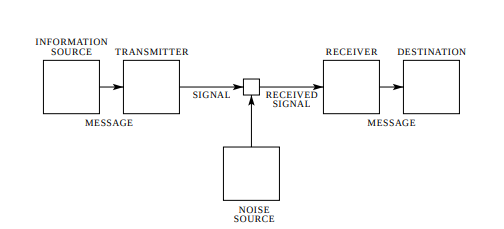
\includegraphics[width=0.65\textwidth]{comunicadorshannon.png}
  \begin{tikzpicture}
    \matrix (A) [matrix of nodes,
    column sep=25pt,
    row sep=30pt,
    nodes={minimum size=35pt}]
    {
      \node[label={[labelst]above:Fonte de\\informação},blocoq] (fonte) {}; &
      \node[label={[labelst]above:Transmissor},blocoq] (trans) {}; &
      \node[minimum size=10pt,blocoq] (conn) {}; &
      \node[label={[labelst]above:Receptor},blocoq] (rec) {}; &
      \node[label={[labelst]above:Destino},blocoq] (dest) {}; \\
      & & \node[label={[labelst]below:Fonte de \\ruído},blocoq] (ruido) {}; \\
    };
    \draw[conecta] (fonte) -- node[pos=0.5,below,labelst,yshift=-20pt] {Mensagem} (trans);
    \draw[conecta] (trans) -- node[pos=0.5,below,labelst] {Sinal} (conn);
    \draw[conecta] (conn) --  node[pos=0.5,below,labelst] {Sinal\\recebido} (rec);
    \draw[conecta] (rec) -- node[pos=0.5,below,labelst,yshift=-20pt] {Mensagem} (dest);
    \draw[conecta] (ruido) -- (conn);
  \end{tikzpicture}
  \fonte{Adaptado de \textcite[p. 380]{MTC}.}
\end{figure}

De acordo com  a TMC, um \textit{gerador de informação} é um objeto capaz de produzir um conjunto $X$ de $n$ eventos com probabilidade de ocorrência $P(X)$, enquanto um \textit{receptor} possui um conjunto $Y$, também com $n$ eventos, com probabilidades associadas $P(Y)$. Durante a transmissão é possível que parte da informação seja perdida devido a ocorrência de ruídos, o que resulta diretamente na modificação dos valores de probabilidade dos elementos recebidos do conjunto $Y$. Reconhecendo portanto os elementos de $X$ e suas probabilidades associadas, espera-se que uma mensagem bem transmitida, ou seja, sem interferência de ruídos, seja aquela cujas probabilidades dos elementos do conjunto $Y$ sejam as mesmas dos elementos do conjunto $X$. Assim, se essas probabilidades forem distintas, podemos concluir que houve perda de informação na transmissão \cite{mathematical}.

De maneira geral, a informação é quantificada de acordo com os recursos físicos necessários para que ela seja representada, ou seja, na capacidade de armazenamento, comunicação e representação de um conjunto $X$ de possíveis informações. Em um computador clássico, por exemplo, armazenamos informações através das unidades binárias chamadas \textit{bits}\footnote{Nome proposto, segundo o artigo original de Shannon por J.W. Turkey \cite{MTC}.}. Dessa forma, os bits são a menor unidade de armazenamento de informação em um computador de arquitetura clássica, podendo representar o estado 1 ou o estado 0 \cite{MTC}.

A combinação desses bits faz com que uma mensagem possa ser armazenada, processada ou transmitida em um computador clássico. Nesse sentido, quão maior, ou ainda, quão mais complexa for a mensagem a se operar, mais bits serão necessários e consequentemente mais recursos físicos para a representação destes.

A descrição da arquitetura de um computador quântico esbarra no mesmo princípio daquela de um computador clássico, ou seja, em sua unidade fundamental de armazenamento de informação. De maneira análoga ao computador clássico, que utiliza como unidade de informação o bit, o computador quântico utilizará o \textit{qubit} (ou q-bit, ou ainda, quantum bit).

Um qubit, ou bit quântico, pode ser produzido de maneiras distintas\footnote{Qubits podem ser fisicamente criados utilizando, por exemplo, spins de átomos presos em uma armadilha. Essa armadilha pode ser do tipo óptica ou até mesmo magnética. É possível também polarizar fótons para sua obtenção. A determinação do método é definida principalmente pelo mecanismo que melhor conseguir isolar o qubit, já que este é facilmente influenciado pelo ambiente externo \cite{materialdidaticomecquantica}.}, porém nosso foco de estudo está nas suas propriedades. Um qubit é uma unidade com propriedades quânticas que atua sob o regime de superposição de estados. Isso significa que ele consegue armazenar simultaneamente mais de um estado de informação, diferente do bit clássico que armazena apenas um dos estados por vez. Decorre desta propriedade a maior capacidade de operar a informação em comparação aos mecanismos clássicos segundo apresentado na Tabela~\ref{tabelabit}.

\begin{table}[ht]
  \centering
  \caption{Comparação entre a quantidade de bits clássicos e quânticos necessários para se operar uma informação.}\label{tabelabit}
  \begin{tabular}{ccc}
    \toprule
    \thead{Quantidade \\ de bytes \\ (informação)} & \thead{Quantidade \\ de bits clássicos} & \thead{Quantidade \\ de qubits} \\
    \midrule
    1         & 8            & 3  \\
    \num{e6}  & \num{8.3e6}  & 23 \\
    \num{e12} & \num{8.8e12} & 43 \\
    \bottomrule
  \end{tabular}
  \fonte{Elaborada pelo autor.}
\end{table}

De modo a generalizar a comparação entre bits classicos e quânticos, podemos estabelecer a relação:
\begin{equation} \label{bitvsqubit}
n\, \text{qubits} = 2^{n}\,\text{bits}.
\end{equation}

Portanto, podemos concluir que menos qubits são necessários para operar a informação, em comparação ao bit clássico, o que está diretamente relacionado com a velocidade e com a capacidade de realização deste.

Segundo \textcite{CompInfoQuantica} e \textcite{dwave}, a devida construção de um computador de arquitetura quântica foi precedida pelos eventos descritos a seguir:

\begin{description}
  \item[1985] David Deustch propõe matematicamente o primeiro computador quântico universal;
  \item[1994] Peter Shor cria o primeiro programa essencialmente quântico, ou seja, ele não poderia ser executado em um computador clássico. Este programa, conhecido como Algoritmo de Shor, reduziria o tempo de fatoração de números grandes de possíveis meses para apenas segundos caso fosse utilizado em um computador real de arquitetura quântica;
  \item[1999] O MIT apresenta o primeiro protótipo de um computador quântico real;
  \item[2007] A empresa D-Wave apresenta o primeiro computador essencialmente quântico.
\end{description}

Apesar de na atualidade processadores quânticos existirem e operarem\footnote{Atualmente a IBM possuí um processador que opera com 433 qubits simultâneos, o \textit{Osprey}, anunciado em novembro de 2022 \cite{osprey}.}, ainda estamos distantes da efetiva implementação comercial de um computador quântico. Podemos utilizar de exemplo, o fato de que apesar de possuirmos um análogo para a TMC de Shannon em um computador quântico\footnote{Em 1995, Benjamin Schumacher propõe com êxito um análogo quântico para o TMC \cite{benschu}.}, ainda não temos um análogo quântico para um sistema submetido a ruídos na transmissão\footnote{Contudo, foi desenvolvida a teoria de correção de erros quânticos que permite que computadores quânticos possam operar na presença de ruídos e que a informação quântica seja transmitida de maneira confiável \cite{chuang}}\cite{chuang}.

Portanto, o estudo de simulações de sistemas de informação quânticos se faz necessário para aperfeiçoamento desses mecanismos e ainda para o desenvolvimento da própria Física, visto que o avanço da compreensão da utilização da mecânica quântica atrelado ao conceito de informação, possibilita a compreensão da natureza de maneira cada vez mais complexa, sem a necessidade de aproximações e simplificações \cite{chuang}.

Devido aos recursos de simulação, podemos utilizar um computador de arquitetura clássica para simular tanto um qubit quanto os circuitos lógicos necessários para a realização de operações com a informação quântica, a título do estudo, por exemplo, dos efeitos de ruídos na transmissão da informação quântica conforme propomos nesse trabalho. Nesse sentido, os próximos capítulos irão introduzir conceitos sobre informação quântica e mecânica quântica para a compreensão do desenvolvimento do trabalho.
             % INTRODUÇÃO
%%%  _____               _
%%% |_   _|__  ___  _ __(_) __ _
%%%   | |/ _ \/ _ \| '__| |/ _` |
%%%   | |  __/ (_) | |  | | (_| |
%%%   |_|\___|\___/|_|  |_|\__,_|
%%%
%%% TCC de Bianca Miyabe Santos Freitas
%%% Licenciatura em Física - UFSCar, Sorocaba
%%%

\chapter{Fundamentação Teórica}

Conforme descrito no Capítulo de Introdução, para o estudo da Computação Quântica e da Informação Quântica são necessários alguns recursos provenientes da Mecânica Quântica, bem como a construção de análogos quânticos para o processamento dessa informação. As seções a seguir apresentarão a fundamentação teórica e os recursos matemáticos necessários para o desenvolvimento da simulação proposta na Metodologia.

\section{Conceitos básicos de Álgebra Linear}
A Álgebra Linear é o estudo dos vetores que descrevem um espaço e consequentemente das operações nesses espaços vetoriais. Para o desenvolvimento desse trabalho, serão necessários reconhecer as notações descritas na Tabela~\ref{tab:notação}.

\begin{table}[ht!]
  \centering
  \caption{Notações utilizadas nas operações de Mecânica Quântica e sua respectiva descrição. O estilo das notações é conhecido como Notação de Dirac para Álgebra Linear.}\label{tab:notação}
  \begin{tabular}{cl}
    \toprule
    {\textbf{Notação}}                 & {\textbf{Descrição}}                                                 \\
    \midrule
    $\ket{\psi}$                       & Vetor conhecido como \textit{ket}                                    \\
    $\bra{\psi}$                       & Vetor dual de um \textit{ket} conhecido como \textit{bra}            \\
    $\braket{\psi\vert\varphi}$        & Produto interno entre os vetores $\ket{\psi}$ e $\ket{\varphi}$      \\
    $\ket{\psi} \otimes \ket{\varphi}$ & Produto tensorial entre os vetores $\ket{\psi}$ e $\ket{\varphi}$    \\
    $\ket{\psi}\ket{\varphi}$          & Abreviação do produto tensorial entre $\ket{\psi}$ e $\ket{\varphi}$ \\
    $A^*$                              & Conjugado complexo da matriz \(A\)                                   \\
    \bottomrule
  \end{tabular}
  \fonte{Adaptada de \textcite{chuang}.}
\end{table}

A descrição da Mecânica Quântica é feita tomando como base um espaço vetorial chamado \textit{Espaço de Hilbert} $\mathcal{H}$, sendo este um espaço complexo, vetorial e linear. Um \textit{ket} é um vetor arbitrário de $\mathcal{H}$, com representação descrita por:
\begin{equation}\label{eq:ketpsi}
  \ket{\psi} = [\psi_1,...,\psi_n]^T \in \mathcal{H}.
\end{equation}

Todo \textit{ket} possui um vetor dual, ou conjugado complexo que também pertence à $\mathcal{H}$, chamado de \textit{bra}, de modo que:
\begin{equation}\label{eq:brapsi}
  \bra{\psi} = [\psi_1^*,...,\psi_n^*] \in \mathcal{H}.
\end{equation}

O produto tensorial entre dois \textit{kets} \(\ket{\psi}\) de dimensão \(m\) e \(\ket{\varphi}\) de dimensão \(n\) é definido por:
\begin{equation}\label{eq:tensorket}
\ket{\psi} \otimes \ket{\varphi} = \ket{\psi}\ket{\varphi} =\ket{\psi \varphi} =\begin{pmatrix}\psi_1 \varphi_1 \\ \psi_1 \varphi_2 \\ \vdots \\ \psi_1 \varphi_n \\ \psi_2 \varphi_1 \\ \psi_2 \varphi_2 \\ \vdots \\ \psi_2 \varphi_n \\ \vdots \\ \psi_m \varphi_2 \\ \psi_m \varphi_2 \\ \vdots \\ \psi_m \varphi_n\end{pmatrix}.
\end{equation}

\todo[inline]{Que tal assim?}

\begin{equation}\label{eq:tensorket}
  \begin{split}
    \ket{\psi} \otimes \ket{\varphi} &= \ket{\psi}\ket{\varphi} =\ket{\psi \varphi} = \\
    &=\scalebox{0.9}{\(\begin{pmatrix}\psi_1 \varphi_1 & \psi_1 \varphi_2 & \cdots & \psi_1 \varphi_n & \psi_2 \varphi_1 & \psi_2 \varphi_2 & \cdots & \psi_2 \varphi_n & \cdots & \psi_m \varphi_2 & \psi_m \varphi_2 & \cdots & \psi_m \varphi_n\end{pmatrix}^{T}\)}.
  \end{split}
\end{equation}
Podemos também realizar o produto tensorial de duas matrizes \(A\in\mathbb{C}^{m{\times}n}\) e \(B\in\mathbb{C}^{p{\times}q}\), de modo que:
\begin{equation}\label{eq:tensormatrix}
  A \otimes B = \begin{pmatrix}
                  A_{11} B  & A_{12} B  & \cdots & A_{1 n} B \\
                  A_{21} B  & A_{22} B  & \cdots & A_{2 n} B \\
                  \vdots    & \vdots    & \ddots & \vdots    \\
                  A_{m 1} B & A_{m 2} B & \cdots & A_{m n} B
                \end{pmatrix}_{m p \times n q}.
              \end{equation}

O conjugado complexo de uma matriz é definido como a matriz transposta dos seus elementos conjugados, de modo que:
\begin{equation}\label{eq:conjugadomatrix}
  A^{\!*} = \begin{pmatrix}
                a & b \\
                c & d
          \end{pmatrix}^{\!\!\!*} =
          \begin{pmatrix}
            a^{*} & c^{*} \\
            b^{*} & d^{*}
          \end{pmatrix}.
      \end{equation}

Os recursos apresentados acima, serão utilizados ao longo do trabalho e principalmente na descrição da Seção~\ref{Mecanicaquantica}.


\section{Mecânica Quântica}\label{Mecanicaquantica}

\section{Qubits}

As definições de qubits descritas nesse tópico baseiam-se principalmente nas ideias apresentadas por \textcite{chuang} e \textcite{CompInfoQuantica}.

Qubits são elementos fundamentais da computação quântica. Eles são usados para representar informações binárias (zeros e uns) e são capazes de armazenar e processar muito mais informações que os bits convencionais usados na computação clássica. Isso é possível graças ao fato de que, enquanto os bits tradicionais podem estar em dois estados (ligado ou desligado), os qubits podem estar em um estado de superposição, o que permite que eles representem simultaneamente vários estados ou informações diferentes. Isso significa que os qubits podem armazenar muito mais informação em um espaço muito menor conforme salientado na Tabela~\ref{tabelabit}.

Podemos começar a descrição de um qubit como uma superposição dos estados quânticos $\ket{0}$ e $\ket{1}$, de modo a representá-los pela combinação linear dada por
\begin{equation}\label{eq:psi}
\ket{\psi} = \alpha \ket{0} + \beta \ket{1},
\end{equation}
com $\alpha$ e $\beta$ parametrizados por \(\alpha^{2} + \beta^{2} = 1\).

Os números $\alpha$ e $\beta$ são complexos e determinam as amplitudes probabilísticas da obtenção dos estados quânticos. O estado descrito por $\ket{\psi}$ é uma superposição dos estados quânticos $\ket{0}$ e $\ket{1}$, ou seja, seguindo os postulados da mecânica quântica, o qubit pode existir num estado contínuo entre $\ket{0}$ e $\ket{1}$ porém, ao ser medido, colapsando o sistema, retornará apenas os valores de $\ket{0}$ ou $\ket{1}$ com as probabilidades $\alpha$ e $\beta$ associadas.

Um recurso para visualizar o comportamento de qubits é sua representação geométrica chamada de Esfera de Boch. Como entidades quânticas não são observáveis diretamente e frequentemente são expressas por recursos matemáticos, a visualização da superposição dos estados de um qubit utilizando a Esfera de Boch facilita, ainda que ligeiramente, sua compreensão.

Em primeiro lugar, vale lembrar que o qubit, descrito por $\ket{\psi}$, está parametrizado e podemos reescrever~\eqref{eq:psi} em coordenadas polares
\begin{equation}
\ket{\psi}=e^{i \gamma}\Biggl(\cos \frac{\theta}{2}\ket{0}+e^{i \varphi} \sen \frac{\theta}{2}\ket{1}\Biggr).
\end{equation}
O termo \(e^{i\gamma}\) não possui efeitos observáveis na representação geométrica e portanto, podemos simplificar a equação acima, obtendo
\begin{equation}\label{eq:coordpolarpsi}
\ket{\psi}=\Biggl(\cos \frac{\theta}{2}\ket{0}+e^{i \varphi} \sen \frac{\theta}{2}\ket{1}\Biggr),
\end{equation}
com $\theta$ e $\varphi$ sendo números reais correspondentes aos ângulos entre os eixos $z, y$ e $y, x$ respectivamente, conforme a
Figura~\ref{fig:bloch}.

\begin{figure}[ht!]
\centering
\caption{Representação gráfica de um qubit como um ponto sob a superfície da Esfera de Boch.}\label{fig:bloch}
% Adaptado de https://tex.stackexchange.com/questions/345420/how-to-draw-a-bloch-sphere
\begin{blochsphere}[radius=3cm,rotation=-110,opacity=0]
  \drawLongitudeCircle[]{-110};
  \drawLatitudeCircle[style={dashed}]{0};
  \labelLatLon{ket0}{90}{0};
  \labelLatLon{ket1}{-90}{0};
  \labelLatLon{ketminus}{0}{180};
  \labelLatLon{ketplus}{00}{0};
  \labelLatLon{ketpluspi2}{0}{-90};  % Longitude seems to be defined in the "wrong" direction, hence the minus
  \labelLatLon{ketplus3pi2}{0}{-270};
  \labelLatLon{psi}{45}{-45};

  \draw[-latex] (0,0) -- (ket0) node[pontinho=blue] {} node[below right,inner sep=.5mm] at (ket0) {$z$} node[above,inner sep=.5mm] at (ket0) {$\ket{0}$};
  \draw[-latex,dashed,opacity=0.2] (0,0) -- (ket1);
  \node[pontinho=blue] at (ket1) {} node[below,inner sep=.5mm] at (ket1) {$\ket{1}$};
  \draw[-latex] (0,0) -- (ketplus) node[below,inner sep=.5mm] at (ketplus) {$x$};
  \draw[-latex] (0,0) -- (ketpluspi2) node[below,inner sep=.5mm] at (ketpluspi2) {$y$};
  \draw[-latex] (0,0) -- (psi) node[pontinho=blue] {} node[above] {$\ket{\psi}$};

  \coordinate (origin) at (0,0);
  {
    \setDrawingPlane{0}{0}
    \draw[current plane,dashed] (0,0) -- (-90+45:{cos(45)*3cm}) coordinate (psiProjectedEquat) -- (psi);
    \pic[current plane,draw,fill=orange!20,fill opacity=.5,text opacity=1,pic text=$\varphi$,angle eccentricity=2.2,left]{angle=ketplus--origin--psiProjectedEquat};
  }
  { \setLongitudinalDrawingPlane{45}
    \pic[current plane,draw,fill=orange!20,fill opacity=.5,text opacity=1,pic text=$\theta$,angle eccentricity=1.5]{angle=psi--origin--ket0};
  }
\end{blochsphere}
% 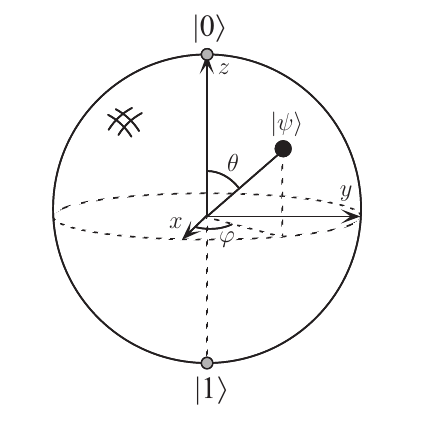
\includegraphics[width=0.5\linewidth]{boch.png}
\fonte{Adaptado de \textcite{chuang}.}
\end{figure}

%EXPLICAR COMO FUNCIONA O ARMAZENAMENTO DE INFORMAÇÃO NO QUBIT E COMO FUNCIONA A MEDIDA DE UM ESTADO

\section{Operadores Quânticos}

Na Mecânica Quântica, um \textit{Operador Quântico} é um objeto matemático que representa uma propriedade física observável de um sistema quântico. Eles são fundamentais para a teoria quântica pois fornecem uma maneira de descrever e prever os resultados de medidas em sistemas quânticos. Eles são representados por matrizes ou operadores lineares que pertencem a um espaço de Hilbert \(\mathcal{H}\) e são equivalentes às portas lógicas na computação clássica, ou seja, são implementadas como operadores quânticos que atuam em um ou mais qubits. As próximas seções serão utilizadas para explicar os principais operadores/portas lógicas quânticas e como eles atuam em um qubit \cite{jorcuvich}.

\subsection{Matrizes de Pauli}\label{sec:pauli}

Segundo \textcite{chuang}, matrizes de Pauli são um conjunto de três matrizes hermitianas e unitárias, amplamente utilizadas na computação quântica. As matrizes são denotadas por $\sigma_x$, $\sigma_y$ e $\sigma_z$, e são definidas por:
\begin{equation}
\sigma_x=\begin{pmatrix}
0 & 1 \\
1 & 0
\end{pmatrix}, \quad \sigma_y=\begin{pmatrix*}[r]
0 & -i \\
i & 0
\end{pmatrix*}, \quad \sigma_z=\begin{pmatrix*}[r]
1 & 0 \\
0 & -1
\end{pmatrix*}.
\end{equation}
As matrizes $\sigma_x$, \(\sigma_{y}\) e \(\sigma_{z}\) são também conhecidas como a matrizes de Pauli X, Pauli Y e Pauli Z, respectivamente. As matrizes de Pauli formam a base do espaço de Hilbert de um único qubit, e podem ser usadas para construir operadores mais complexos que atuam em múltiplos qubits.

\subsection{Porta Lógica Controlled-NOT Quântica}\label{sec:cnot}

As matrizes de Pauli são frequentemente usadas na construção de portas lógicas quânticas. A porta NOT quântica, por exemplo, é usada para inverter o estado de um qubit e é construída a partir da matriz de Pauli X. A porta Controlled-NOT Quântica, ou \(\CNOT\), que é usada para realizar operações lógicas em dois qubits, também é construída a partir de uma combinação das matrizes de Pauli X, Y e Z, além da identidade \cite{CompInfoQuantica}. Esta é uma propriedade geral das portas lógicas quânticas: elas podem ser construídas a partir de matrizes que são combinações das matrizes de Pauli e da matriz de identidade.

A matriz que representa a porta \(\CNOT\) é dada por:
\begin{equation}\label{eq:cnot}
\CNOT = \begin{pmatrix}
1 & 0 & 0 & 0 \\
0 & 1 & 0 & 0 \\
0 & 0 & 0 & 1 \\
0 & 1 & 1 & 0
\end{pmatrix} 
\end{equation}

A porta lógica \(\CNOT\) é usada para implementar operações condicionais e permutações entre qubits, sendo usada para criar circuitos lógicos quânticos mais complexos como uma versão geral da porta NOT clássica, pois ela pode ser aplicada a todos os qubits e não apenas a dois. Na porta \(\CNOT\), o qubit de controle é usado para controlar o estado do qubit alvo. Se o qubit de controle estiver em $\ket{1}$, o estado do qubit alvo será invertido, mas se o qubit de controle estiver em $\ket{0}$, o estado do qubit alvo não será alterado \cite{chuang}.


\subsection{Porta Lógica Hadamard Quântica}\label{sec:had}

A Porta Lógica Hadamard Quântica \(\HAD\) é uma porta lógica quântica que transforma o estado de um qubit em seu estado oposto com 50\% de probabilidade associada ao estado. Ela pode ser usada para realizar operações de entrelaçamento entre qubits, o que permite a implementação de algoritmos quânticos como o emaranhamento e o teletransporte quântico. Seu desenvolvimento teve como objetivo permitir o controle preciso de qubits em circuitos quânticos \cite{jorcuvich}. Ela é representada por uma matriz 2x2, definida como:

\begin{equation}
\HAD= \frac{1}{\sqrt{2}} \begin{pmatrix*}[r]
1 & 1 \\
1 & -1
\end{pmatrix*}
\end{equation}


\section{Emaranhamento Quântico}

%O emaranhamento quântico é o fenômeno pelo qual partículas elementares, como fótons, elétrons e outras, ligam-se entre si de tal maneira que um objeto passa a ter quase que uma única identidade. Neste estado, um objeto passa a ter propriedades que estão além dos limites da mecânica quântica. Em outras palavras, o emaranhamento quântico é um estado no qual duas partículas interagem de forma tal que elas compartilham o mesmo estado e não podem ser descritas independentemente. Por exemplo, dois fótons entrelaçados podem ser entendidos como uma única partícula, mesmo que eles estejam distantes um do outro. O emaranhamento quântico pode ser usado para criar ligações entre partículas e objetos distantes, o que abre portas para o desenvolvimento de novas tecnologias, como a computação quântica.
%
%Etapas do Emaranhamento Quântico de Qubits
%
%\begin{itemize}
%\item 1. Preparação:  O primeiro passo é preparar os qubits individuais. Isso pode ser feito carregando os qubits em computadores quânticos ou usando dispositivos quânticos especializados, como lasers.
%
%\item 2. Entrelaçamento: Em seguida, os qubits são entrelaçados, o que significa que eles são interconectados de modo que as informações entre eles sejam compartilhadas. Isso pode ser feito usando técnicas como a interferência quântica.
%
%\item 3. Operações: Uma vez que os qubits estão entrelaçados, as operações quânticas podem ser realizadas neles. As operações podem incluir a realização de computações quânticas complexas, o armazenamento de informações quânticas ou o envio de informações entre qubits.
%
%\item 4.Saída: Por fim, os qubits podem ser desentrelaçados para obter a saída desejada. Isso pode ser feito usando técnicas como a interferência quântica inversa. A saída pode incluir informações codificadas nos qubits, como um resultado de uma computação quântica.
%
%\end{itemize}



\section{Teletransporte Quântico}
%O  Teletransporte Quântico
%
%O Teletransporte Quântico é um processo de transferência de informação quântica entre dois pontos, usando mecanismos quânticos. Essa transferência pode ocorrer quase instantaneamente, independentemente da distância entre os dois pontos.
%O Teletransporte Quântico é baseado em princípios da mecânica quântica, que descrevem como os estados quânticos podem ser compartilhados entre partículas e aplicados aos sistemas de informação. O Teletransporte Quântico foi descoberto pela primeira vez pela física austríaca Anton Zeilinger, em 1998. Ela escobriu que, usando um fenômeno conhecido como entrelaçamento quântico, é possível transferir informação instantaneamente entre dois pontos. O princípio básico do teletransporte quântico é que dois partículas, como elétrons, átomos ou fótons, podem ser entrelaçados, ou ligados entre si. Quando isso acontece, qualquer mudança na configuração de uma partícula será imediatamente refletida na outra, mesmo que elas estejam separadas por uma distância enorme. Isso significa que informação pode ser enviada instantaneamente entre dois pontos distantes.
%
%Embora o teletransporte quântico ainda esteja em fase experimental, já foi usado para transferir informações básicas como posição, polarização e estado de spin entre dois pontos separados. A tecnologia ainda precisa desenvolver muito antes de poder ser usada para transferir informações mais complexas, como imagens ou dados.
%
%Na prática, o Teletransporte Quântico permite que um estado quântico seja transferido de um lugar para outro, sem que nenhuma informação seja transferida entre os locais. Isso significa que um estado quântico pode ser transmitido de uma parte do universo para outra sem que nenhuma informação seja trocada entre eles.
%O Teletransporte Quântico é usado em diversas áreas científicas, como criptografia, computação quântica, comunicação segura e muito mais. Também pode ser usado para transferir informações confidenciais de um lugar para outro, impedindo que terceiros interceptem a informação.


\section{Protocolo de Teletransporte Quântico}

A descrição deste protocolo foi baseada em \textcite{chuang, jorcuvich, CompInfoQuantica, benschu}. A realização de um protocolo de Teletransporte Quântico consiste, essencialmente, em uma série de operações que possuem por objetivo principal fazer com que uma mensagem, ou na linguagem quântica, um estado quântico, se teletransporte entre dois pontos distintos fisicamente.
Como em qualquer outra operação computacional é necessária a existencia de um circuito lógico, nesse caso quântico, que media as operações. Esse circuito consistirá nas combinações das portas lógicas \(\CNOT\), Haddamard, portas de medição e as portas \(\XXX\) e \(\ZZZ\) conforme a Figura~\ref{fig:protocoloteletransporte}.

\begin{figure}[ht!]
\centering
\caption{Protocolo de Teletransporte Quântico mediado pelo circuito com as portas \(\CNOT\), Hadamard, bedição aplicadas no Local \(A\) e as portas \(\XXX\) e \(\ZZZ\) aplicadas no Local \(B\).}\label{fig:protocoloteletransporte}
\begin{quantikz}[slice style=blue]
\lstick{$\ket{\psi}$} & \qw & \qw & \qw \slice{$\ket{\psi_0}$} & \ctrl{1} \slice{$\ket{\psi_1}$} & \gate{H} \slice{$\ket{\psi_2}$} & \meter{$M_1$} & \cw  & \cw & \cwbend{2}\\
\lstick{$\ket{q_x}$} & \gate{H}\gategroup[2,steps=2,style={dashed,rounded corners,fill=blue!20, inner xsep=2pt}, background,label style={label position=below,anchor=north,yshift=-0.2cm}]{{Emaranhamento}} & \ctrl{1} & \midstick[2]{$\ket{\beta_{00}}$} \qw & \targ{} & \qw & \meter{$M_2$} & \cwbend{1} \\
\lstick{$\ket{q_y}$} & \qw & \targ{} \arrow{r} &  & \qw & \qw & \qw & \gate{X} & \qw & \gate{Z} &  \qw\rstick{$\ket{\psi}$}
\end{quantikz}
\fonte{Adaptado de }
\end{figure}

No inicio do protocolo é necessário que tenhamos um par de qubits emaranhados nas bases de Bell, no estado $\ket{\beta_{00}}$, que podemos representar pela expressão
\begin{equation}\label{eq:bell00}
 \ket{\beta_{00}} = \frac{\ket{00} + \ket{11}}{\sqrt{2}}.
\end{equation}

Um dos qubits do par emaranhado em~\eqref{eq:bell00} é mantido em \(A\) e o outro necessariamente precisa estar em \(B\) para que exista um canal de comunicação entre essas partes. Além do par emaranhado, em \(A\) teremos o estado quântico a ser enviado, ou seja sua mensagem dada por $\ket{\psi}$, segundo a Equação~\eqref{eq:psi}.
% \begin{equation}\label{psi}
%  \ket{\psi} = \alpha \ket{0} + \beta \ket{1}.
% \end{equation}
De posse do par emaranhado e da mensagem, o protocolo é iniciado com a aplicação da porta \(\CNOT\) entre $\ket{\psi}\ket{\beta_{00}}$, que chamaremos de $\ket{\psi_0}$. A porta \(\CNOT\) possui como alvo o qubit $\ket{q_y}$ e como qubit de controle $\ket{q_x}$. Isso indica que a porta \(\CNOT\) irá modificar $\ket{q_y}$ de acordo com o estado de $\ket{q_x}$ de modo que:

\todo[inline]{De modo que\ldots}


\begin{theo}{Operação \(\CNOT\)}{cnot}
  A operação \(\CNOT\):
  \begin{enumerate}[label=\roman*.,left=0pt]
    \item Inverte o qubit alvo, caso o qubit de controle esteja no estado $\ket{1}$;
    \item Não realiza operação alguma no qubit alvo, caso o controle esteja no estado $\ket{0}$.
  \end{enumerate}
\end{theo}

Dessa maneira, aplicando a Definição~\ref{def:cnot} no estado dado por $\ket{\psi_0}$
\begin{align}\label{eq:cnotpsi0}
  \CNOT \ket{\psi_0} &= \CNOT \ket{\psi} \ket{\beta_{00}} \nonumber \\
                     &= \CNOT \frac{1}{\sqrt{2}} \Bigl[ \alpha \ket{0} \bigl( \ket{00} + \ket{11} \bigr) + \beta \ket{1} \bigl( \ket{00} + \ket{11} \bigr)\Bigr] \nonumber \\
                     &= \frac{1}{\sqrt{2}} \Bigl[\alpha \ket{0} \bigl( \ket{00} + \ket{11} \bigr) + \beta \ket{1} \bigl( \ket{10} + \ket{01} \bigr) \Bigr].
\end{align}

A operação descrita pela Equação~\eqref{eq:cnotpsi0} resulta no estado que chamaremos de $\ket{\psi_1}$ e neste, segundo o circuito da Figura~\ref{fig:protocoloteletransporte}, deve-se aplicar a porta Hadamard, descrita na Definição~\ref{def:hadamard}.

\begin{theo}{Operação Hadamard}{hadamard}
  A operação Hadamard deve:
  \begin{enumerate}[label=\roman*.]
    \item Aplicar no estado 0 a operação $\frac{1}{\sqrt{2}} \bigl(\ket{0}+\ket{1}\bigr)$;
    \item Aplicar no estado 1 a operação $\frac{1}{\sqrt{2}} \bigl(\ket{0}-\ket{1}\bigr)$.
  \end{enumerate}
\end{theo}

Aplicando portanto a Definição~\ref{def:hadamard} em $\ket{\psi_1}$, teremos:
\begin{equation}\label{eq:hadamartpsi2}
 \HAD \ket{\psi_1} = \Biggl( \frac{1}{\sqrt{2}}\Biggr)^{\!\!2} \Bigl[ \alpha \bigl( \ket{0} + \ket{1} \bigr)\bigl( \ket{00} +\ket{11} \bigr)+ \beta \bigl( \ket{0} - \ket{1} \bigr) \bigl( \ket{10} + \ket{01} \bigr) \Bigr].
\end{equation}

O estado obtido em \eqref{eq:hadamartpsi2} pode ser identificado como $\ket{\psi_2}$, evidenciando-se os estados emaranhados deste ao organizá-lo da seguinte maneira:
\begin{equation}\label{eq:psi2}
 \ket{\psi_2} = \frac{1}{2} \Bigl[ \ket{00} \bigl( \alpha \ket{0} + \beta \ket{1} \bigr) + \ket{01} \bigl( \alpha \ket{1} + \beta \ket{0} \bigr) + \ket{10} \bigl( \alpha \ket{0} - \beta \ket{1} \bigr) + \ket{11} \bigl( \alpha \ket{1} - \beta \ket{0} \bigr) \Bigr].
\end{equation}

O próximo passo do protocolo consiste em realizar medidas em ambos os qubits presentes em \(A\). Essas medidas farão com que os estados quânticos sejam colapsados e deixem de coexistir, passando a ser considerados clássicos. As medidas possíveis de serem obtidas em \(A\) são apresentadas na Tabela~\ref{tab:medidas}.

\begin{table}[ht!]
  \centering
  \caption{Possíveis resultados das medidas realizadas nos qubits presentes em \(A\) no estado quântico $\ket{\psi_2}$.}\label{tab:medidas}
  \begin{tabular}{cc}
    \toprule
    {\textbf{Medida realizada}} & {\textbf{Estado quântico associado}}\\
    \midrule
    $\ket{00}$   & $\bigl( \alpha \ket{0} + \beta \ket{1} \bigr)$\\
    $\ket{01}$   & $\bigl( \alpha \ket{1} + \beta \ket{0} \bigr)$\\
    $\ket{10}$   & $\bigl( \alpha \ket{0} - \beta \ket{1} \bigr)$\\
    $\ket{11}$   & $\bigl( \alpha \ket{1} - \beta \ket{0} \bigr)$\\
    \bottomrule
  \end{tabular}
  \fonte{Elaborada pelo autor.}
\end{table}

Os valores dos estados medidos em \(A\), são enviados via canal clássico até \(B\) que, devido ao emaranhamento com o qubit operado em \(A\), terá seu colapso consequentemente em seu estado quântico associado, segundo a Tabela~\ref{tab:medidas}.

A última etapa do protocolo, ocorre em \(B\), na tentativa de reconstruir a mensagem original, nesse momento já inexistente, que estava em \(A\). Nessa última etapa, serão utilizadas (ou não) as portas lógicas \(\XXX\) e \(\ZZZ\), cujas operações fazem parte das Definições~\ref{def:X} e~\ref{def:Z}

\begin{theo}{Operação \(\XXX\)}{X}
A porta lógica quântica \(\XXX\) deve trocar os estados quânticos, ou seja, torná-lo 1 quando este for 0 e torná-lo 0, quando este for 1.
\end{theo}

\begin{theo}{Operação \(\ZZZ\)}{Z}
A porta lógica quântica \(\ZZZ\) deve inverter a fase do estado quântico, ou seja, torná-la negativa quando esta for positiva e torná-la positiva quando esta for negativa.
\end{theo}

A aplicação das portas dependerá do resultado da medida enviado por \(A\), seguindo o estipulado na Tabela~\ref{tab:acao-das-portas}. Com isso, o protocolo se encerra e a mensagem é teletransportada do ponto \(A\) para o ponto \(B\), sem que nenhum teorema da física quântica seja violado.

\begin{table}[ht!]
  \centering
  \caption{Aplicação das portas lógicas quânticas, de acordo com a medida da informação enviada por \(A\).}\label{tab:acao-das-portas}
  \begin{tabular}{cp{0.6\linewidth}}
    \toprule
    \textbf{Resultado medido} & \textbf{Ação} \\
    \midrule
    $\ket{00}$ & Nenhuma porta deve ser aplicada e o estado colapsado em \(B\) é exatamente o mesmo da mensagem enviada em $\ket{\psi}$ \\
    $\ket{10}$ & Apenas a porta \(\ZZZ\) deve ser aplicada \\
    $\ket{01}$ & Apenas a porta \(\XXX\) deve ser aplicada \\
    $\ket{11}$ & Tanto a porta \(\XXX\) quanto a porta \(\ZZZ\) devem ser aplicadas \\
    \bottomrule
  \end{tabular}
\end{table}


\section{Algoritmo do protocolo de Teletransporte}

Descrição das etapas para o protocolo de teletransporte

\begin{enumerate}
\item Determinar as funções que descrevem os qubits a serem emaranhados
	\begin{itemize}
	\item qubit \(x\)
	\item qubit \(y\)
	\end{itemize}
\item Determinas as matrizes que descrevem as portas utilizadas no emaranhamento
	\begin{itemize}
	\item Porta Hadamard
	\item Porta \(\CNOT\)
	\item Matriz Identidade
	\end{itemize}
\item Determinar as operações entre os qubits e as portas e a ordem de realização para o emaranhamento
	\begin{itemize}
	\item Produto tensorial entre qubit \(x\) e qubit \(y\) $\rightarrow$ qubit \(xy\)
	\item Produto tensonial entre Porta Haddamard e Matriz Identidade $\rightarrow {\HAD} \otimes$ I
	\item Multiplicação entre qubit \(xy\) e ${\HAD} \otimes I \rightarrow {\HAD} xy$
	\item Multiplicação entre \({\HAD} xy\) e a Porta \(\CNOT \rightarrow\beta _{00}\)
	\end{itemize}
\item Determinar o qubit a ser enviado
	\begin{itemize}
	\item Definir a entrada de dados feita pelo usuário
	\item Verificar a possibilidade de acordo com a normalização $\alpha + \beta =1$
	\end{itemize}
\item Aplicar a porta CNOT
	\begin{itemize}
	\item Verificar a condição lógica de aplicação da porta \(\CNOT\)
	\item Aplicar \(\CNOT\) em $\beta_{00} \rightarrow \ket{\psi_1}$
	\end{itemize}
\item Aplicar a porta Hadamard em $\ket{\psi _1} \rightarrow \ket{\psi_2}$
\item Reorganizar e apresentar os estados antes da medição
\item Realizar a medição
	\begin{itemize}
	\item Determinar de modo aleatório qual dos estados serão medidos
	\end{itemize}
\item Apresentar a medição -- transmissão clássica da informação
\item Determinar as operações a serem realizadas de acordo com a medição realizada
\item Apresentar a mensagem original recuperada
\end{enumerate}

\section{Ruídos}
%Os ruídos no teletransporte de informação quântica são aqueles que se produzem durante o processo de transferência de dados quânticos entre dois sistemas distintos. Esses ruídos podem ser de natureza física ou de natureza lógica.
%
%Ruídos físicos são aqueles que se originam de fontes externas, como ruídos elétricos, ruídos electromagnéticos e ruídos térmicos, entre outros. Esses ruídos incluem:
%\begin{itemize}
%\item 1. Interferência de radiação: a radiação eletromagnética proveniente de fontes externas, como estações de rádio e antenas, pode interferir no sinal quântico, distorcendo ou desviando-o de seu destino.
%
%\item 2. Perda de informação: devido às fracas interações entre os componentes da rede quântica, parte da informação pode ser perdida ao longo do caminho, afetando a qualidade e a confiabilidade da transferência.
%
%\item 3. Decoerência: é o fenômeno quântico que pode ocorrer ao longo do caminho, onde a entropia ou o desordem de um sistema aumentam, o que pode levar a erros na recepção de informações.
%
%\item 4. Entropia térmica: o calor presente no ambiente pode levar a alterações nos estados quânticos dos componentes da rede, o que pode levar a erros na transferência de informações.
%
%\item 5. Interferência mecânica: as vibrações e os ruídos mecânicos presentes no local de transferência de informações podem afetar a qualidade e a confiabilidade dos dados transferidos.
%\end{itemize}
%
%Ruídos lógicos são aqueles que surgem a partir do processo de transferência de dados quânticos, como erros de codificação, erros de decodificação e erros de sincronização. Podemos ressaltar:
%\begin{itemize}
%\item 1. Falha na sincronização de tempo: a sincronização de tempo é um passo crítico para o teletransporte quântico. Se os relógios entre os dois locais não estiverem sincronizados, o teletransporte pode falhar.
%
%\item 2. Desequilíbrio de energia: o desequilíbrio de energia pode ocorrer devido aos efeitos de decaimento quântico, o que pode causar a falha do teletransporte.
%
%\item 3. Interferência de campo: o campo de força entre os dois locais pode interferir com os processos quânticos necessários para o teletransporte.
%
%\item 4. Erro de medição: a medição incorreta dos estados quânticos dos dois locais pode resultar em erros que resultam na falha do teletransporte.
%
%\item 5. Vazamento de informação: o vazamento de informação pode levar à perda de informação necessária para o teletransporte quântico.
%\end{itemize}
%
%Além disso, existem também ruídos de medição, que são aqueles que surgem durante as medições quânticas, e ruídos de decoerência, que são aqueles que se produzem durante a decoerência do estado quântico.
%
%Para minimizar os efeitos dos ruídos no teletransporte de informação quântica, é importante realizar a otimização dos protocolos de teletransporte, otimizar o processo de codificação e decodificação e utilizar técnicas de processamento de sinal quântico.
            % FUNDAMENTAÇÃO TEÓRICA
%%%  __  __      _            _
%%% |  \/  | ___| |_ ___   __| | ___
%%% | |\/| |/ _ \ __/ _ \ / _` |/ _ \
%%% | |  | |  __/ || (_) | (_| | (_) |
%%% |_|  |_|\___|\__\___/ \__,_|\___/
%%%
%%% TCC de Bianca Miyabe Santos Freitas
%%% Licenciatura em Física - UFSCar, Sorocaba
%%%

\chapter{Metodologia}
Para iniciar o desenvolvimento de um protocolo de teletransporte quântico, inicialmente realizou-se a dedução do mesmo em forma matricial, conforme apresentado detalhadamente no Apêndice~\ref{app:matricial}

Realizando um exemplo com os valores atribuídos de $\alpha=0,75$ e $\beta=0,25$, teremos que a mensagem a ser enviada é descrita por:
\begin{equation}
\ket{\psi} = 0,75 \begin{pmatrix}
1 \\
0
\end{pmatrix} + 0,25 \begin{pmatrix}
0 \\
1
\end{pmatrix} = \begin{pmatrix}
0,75 \\
0
\end{pmatrix} + \begin{pmatrix}
0 \\
0,25
\end{pmatrix} = \begin{pmatrix}
0,75 \\
0,25
\end{pmatrix}
\end{equation} 

O estado $\ket{\psi_0}$ descrito pela equação~\eqref{eq:psi0} é descrito por:
\begin{equation}
\ket{\psi_0}=\ket{\psi}\ket{\beta_{00}}= \begin{pmatrix}
0,75 \\
0,25  
\end{pmatrix} \left[\frac{1}{\sqrt{2}} \begin{pmatrix}
1 \\
0 \\
0 \\
1
\end{pmatrix}\right]
\end{equation}

Rearranjando os termos segundo~\eqref{eq:psi0cnot}
\begin{equation}
\ket{\psi_0} = \frac{1}{\sqrt{2}}\left\{\left[ \begin{pmatrix}
0,75 \\
0 
\end{pmatrix}  \begin{pmatrix}
1 \\
0 \\
0 \\
1
\end{pmatrix}\right] + \left[ \begin{pmatrix}
0 \\
0,25
\end{pmatrix}  \begin{pmatrix}
1 \\
0 \\
0 \\
1
\end{pmatrix}\right] \right\}
\end{equation}

Explicitando os estados possíveis conforme~\eqref{eq:3qubit}
\begin{equation}
	\begin{split}
\ket{\alpha00} &= \left[ \begin{pmatrix}
0,75 \\
0
\end{pmatrix} \otimes \begin{pmatrix}
1 \\
0
\end{pmatrix} \otimes \begin{pmatrix}
1 \\
0
\end{pmatrix}\right] = \begin{pmatrix}
0,75 & 0 & 0 & 0 & 0 & 0 & 0 & 0
\end{pmatrix}^T \\
\ket{\alpha11} &= \left[ \begin{pmatrix}
0,75 \\
0
\end{pmatrix} \otimes \begin{pmatrix}
0 \\
1
\end{pmatrix} \otimes \begin{pmatrix}
0 \\
1
\end{pmatrix}\right] = \begin{pmatrix}
0 & 0 & 0 & 0,75 & 0 & 0 & 0 & 0
\end{pmatrix}^T \\
\ket{\beta00} &= \left[ \begin{pmatrix}
0 \\
0,25
\end{pmatrix} \otimes \begin{pmatrix}
1 \\
0
\end{pmatrix} \otimes \begin{pmatrix}
1 \\
0
\end{pmatrix}\right] = \begin{pmatrix}
0 & 0 & 0 & 0 & 0,25 & 0 & 0 & 0
\end{pmatrix}^T \\
\ket{\beta11} &=\left[ \begin{pmatrix}
0 \\
0,25
\end{pmatrix} \otimes \begin{pmatrix}
0 \\
1
\end{pmatrix} \otimes \begin{pmatrix}
0 \\
1
\end{pmatrix}\right] = \begin{pmatrix}
0 & 0 & 0 & 0 & 0 & 0 & 0 & 0,25
\end{pmatrix}^T
	\end{split}
\end{equation}
Somando todos os estados possíveis temos:
\begin{equation}
\ket{\alpha00}+\ket{\alpha01}+\ket{\beta00}+\ket{\beta11}= \begin{pmatrix}
0,75 & 0 & 0 & 0,75 & 0,25 & 0 & 0 & 0,25
\end{pmatrix}^T
\end{equation}

Aplicando a porta \(\CNOT\)
\begin{equation}
\begin{split}
		\CNOT (\ket{\alpha00}\ket{\alpha01}\ket{\beta00}\ket{\beta11}) &= \begin{pmatrix}
		1 & 0 & 0 & 0 & 0 & 0 & 0 & 0 \\
		0 & 1 & 0 & 0 & 0 & 0 & 0 & 0 \\
		0 & 0 & 1 & 0 & 0 & 0 & 0 & 0 \\
		0 & 0 & 0 & 1 & 0 & 0 & 0 & 0 \\
		0 & 0 & 0 & 0 & 0 & 0 & 1 & 0 \\
		0 & 0 & 0 & 0 & 0 & 0 & 0 & 1 \\
		0 & 0 & 0 & 0 & 1 & 0 & 0 & 0 \\
		0 & 0 & 0 & 0 & 0 & 1 & 0 & 0 		
		\end{pmatrix} \begin{pmatrix}
		0,75 \\
		0 \\
		0 \\
		0,75 \\
		0,25 \\
		0 \\
		0 \\
		0,25
		\end{pmatrix} = \\
		&=\begin{pmatrix}
		0,75 & 0 &	0 & 0,75 &	0 &	0,25 &	0,25 &	0
		\end{pmatrix}^T
	\end{split}
\end{equation}	
	
Reorganizando o estado $\ket{\psi_1}$ temos, segundo~\eqref{eq:psi1}
\begin{equation}
\ket{\psi_1} = \frac{1}{\sqrt{2}} \left\{ \begin{pmatrix}
0,75 \\
0
\end{pmatrix} \otimes \left[ \begin{pmatrix}
1 \\
0 \\
0 \\
0
\end{pmatrix} + \begin{pmatrix}
0 \\
0 \\
0 \\
1
\end{pmatrix}\right] +  \begin{pmatrix}
0 \\
0,25
\end{pmatrix} \otimes \left[ \begin{pmatrix}
0 \\
0 \\
1 \\
0
\end{pmatrix} + \begin{pmatrix}
0 \\
1 \\
0 \\
0
\end{pmatrix}\right] \right\}
\end{equation}	

Aplicando a porta \(\HAD\)
\begin{equation}
\begin{split}
		\HAD \ket{\psi} &= \frac{1}{\sqrt{2}} \begin{pmatrix*}[r]
		1 & 1 \\
		1 & -1
		\end{pmatrix*} \frac{1}{\sqrt{2}}\left( \begin{pmatrix}
		0,75 \\
		0 
		\end{pmatrix} +  \begin{pmatrix}
		0 \\
		0,25
		\end{pmatrix} \right) = \frac{1}{2} \left[ \begin{pmatrix}
		,75 \\
		0,75 
		\end{pmatrix} + \beta \begin{pmatrix*}[r]
		0,25 \\
		-0,25
		\end{pmatrix*} \right]
  	\end{split}
\end{equation}	

Reorganizando os resultados para definir o estado $\ket{\psi_2}$ temos

\begin{equation}
 \begin{split}
\ket{\psi_2} &=\frac{1}{2} \left\{ \left[\begin{pmatrix}
1 \\
0
\end{pmatrix} \otimes \begin{pmatrix}
1 \\
0
\end{pmatrix}\right] \left[ \begin{pmatrix}
0,75 \\
0
\end{pmatrix} +  \begin{pmatrix}
0 \\
0,25
\end{pmatrix}\right]\right\} \nonumber \\
&+\frac{1}{2} \left\{ \left[\begin{pmatrix}
0 \\
1
\end{pmatrix} \otimes \begin{pmatrix}
0 \\
1
\end{pmatrix}\right] \left[ \begin{pmatrix}
0 \\
0,75
\end{pmatrix} -  \begin{pmatrix}
0,25 \\
0
\end{pmatrix}\right]\right\} \nonumber \\
&+\frac{1}{2} \left\{\left[ \begin{pmatrix}
1 \\
0
\end{pmatrix} \otimes \begin{pmatrix}
0 \\
1
\end{pmatrix}\right] \left[ \begin{pmatrix}
0 \\
0,75
\end{pmatrix} +  \begin{pmatrix}
0,25 \\
0
\end{pmatrix}\right]\right\} \nonumber \\
&+\frac{1}{2} \left\{ \left[ \begin{pmatrix}
0 \\
1
\end{pmatrix} \otimes \begin{pmatrix}
1 \\
0
\end{pmatrix}\right] \left[ \begin{pmatrix}
0,75 \\
0
\end{pmatrix} -  \begin{pmatrix}
0 \\
0,25
\end{pmatrix}\right] \right\}
  \end{split}
\end{equation}	
	
Para reconstruir o estado, aplicando as condições descritas na tabela~\ref{tab:acao-das-portas} teremos:

Se a medida realizada for o estado $\ket{00}$, o estado enviado foi $\ket{\psi} = \begin{pmatrix}
0,75 \\
0
\end{pmatrix} +  \begin{pmatrix}
0 \\
0,25
\end{pmatrix}$	

Se a medida realizada for o estado $\ket{11}$:

\begin{equation}
\begin{pmatrix}
0 \\
0,75
\end{pmatrix} -  \begin{pmatrix}
0,25 \\
0
\end{pmatrix} = \begin{pmatrix}
-0,25 \\
0,75
\end{pmatrix}
\end{equation}

Aplicando \(\XXX\)

\begin{equation}
\begin{pmatrix}
0 & 1 \\
1 & 0
\end{pmatrix} \begin{pmatrix}
-0,25 \\
0,75
\end{pmatrix} = \begin{pmatrix}
0,75 \\
-0,25
\end{pmatrix}
\end{equation}

Aplicando \(\ZZZ\)

\begin{equation}
\begin{pmatrix}
1 & 0 \\
0 & -1
\end{pmatrix}\begin{pmatrix}
0,75 \\
-0,25
\end{pmatrix} = \begin{pmatrix}
0,75 \\
0,25
\end{pmatrix}
\end{equation}`

Portanto o estado recuperado é:

\begin{equation}
\begin{pmatrix}
0,75 \\
0,25
\end{pmatrix} = \begin{pmatrix}
0,75 \\
0
\end{pmatrix} +  \begin{pmatrix}
0 \\
0,25
\end{pmatrix}
\end{equation}

Se a medida realizada for o estado $\ket{10}$:

\begin{equation}
\begin{pmatrix}
0,75 \\
0
\end{pmatrix} -  \begin{pmatrix}
0 \\
0,25
\end{pmatrix} = \begin{pmatrix}
0,75 \\
-0,25
\end{pmatrix}
\end{equation}

Aplicando \(\ZZZ\)

\begin{equation}
\begin{pmatrix}
1 & 0 \\
0 & -1
\end{pmatrix}\begin{pmatrix}
0,75 \\
-0,25
\end{pmatrix} = \begin{pmatrix}
0,75 \\
0,25
\end{pmatrix}
\end{equation}

Por último, se a medida realizada for o estado $\ket{01}$:

\begin{equation}
\begin{pmatrix}
0,25 \\
0
\end{pmatrix} +  \begin{pmatrix}
0 \\
0,75
\end{pmatrix} = \begin{pmatrix}
0,25 \\
0,75
\end{pmatrix}
\end{equation}

Aplicando \(\XXX\)

\begin{equation}
\begin{pmatrix}
0 & 1 \\
1 & 0
\end{pmatrix} \begin{pmatrix}
0,25 \\
0,75
\end{pmatrix} = \begin{pmatrix}
0,75 \\
0,25
\end{pmatrix}
\end{equation}

Todos os estados recuperados são iguais aos estados enviados e portanto a dedução de~\ref{app:matricial} pode ser utilizada como um guia para um programa que automatize tais operações, conforme veremos a seguir.

Para alcançar o objetivo deste trabalho, ou seja, construir uma simulação de um teletransporte quântico, foi necessário inicialmente decidir a linguagem a ser utilizada para o projeto, que nesse caso, foi o Python. Essa escolha foi feita pois, essa linguagem de programação é amplamente utilizada para simular situações físicas e possuí uma série de bibliotecas que permitem desenvolver os mais diversos projetos. As bibliotecas utilizadas no projeto foram a \textit{sympy, numpy, math, sys e random}, e sua utilização será explicitada durante a explicação das etapas do código fonte. Antes de iniciar a construção do código, foi necessário analisar a estrutura de dados que seria utilizada e a escolhida foi a representação matricial. Essa escolha foi fundamentada no fato de que desse modo, as operações ficam mais explicitas, facilitando a compreensão do protocolo.

De posse da estrutura de dados a ser operacionalizada, da linguagem de programação e dos pacotes necessários, foi desenvolvido o código apresentado no Apêndice~\ref{app:protocolo}. Vamos detalhar as operações e correlacioná-las a seguir.

A primeira etapa da elaboração do protocolo consistiu em importar as bibliotecas necessárias e algumas funções dessas bibliotecas como a \textit{TensorProduct} em \textit{sympy.physics.quantum}. Essa função irá facilitar a realização dos produtos tensoriais durante o desenvolvimento do protocolo.

Com as bibliotecas carregadas, a primeira etapa foi a construção das variáveis que descrevem os estados quânticos $\ket{0}$ e $\ket{1}$, elas foram feitas com o auxílio da biblioteca \textit{numpy} e da função\textit{matrix} que cria matrizes à partir de listas. Portando o estado $\ket{0}$ foi definido pela variável \begin{tiny}\textbf{$qbit0= np.matrix([1,0]).transpose()$}\end{tiny} e o estado $\ket{1}$ pela variável \begin{tiny}\textbf{$qbit1= np.matrix([0,1]).transpose()$}\end{tiny}.
Foram estabelecidas também as variáveis que representam os operadores quânticos, para a porta \(\HAD\) criou-se a variável \textit{$H$}, representada por \begin{tiny}\textbf{$H = 1/sqrt(2)*(np.matrix([[1,1], [1,-1]]))$}\end{tiny}, para a porta \(\CNOT\) temos a variável \begin{tiny}\textbf{$CNOT = np.matrix([[1,0,0,0],[0,1,0,0],[0,0,0,1],[0,0,1,0]])$}\end{tiny}, para a porta \(\III\) a variável \begin{tiny}\textbf{$I = np.matrix ([[1,0], [0,1]])$}\end{tiny}, para as matrizes de Pauli \(\XXX\) e \(\ZZZ\) as variáveis \begin{tiny}\textbf{$X = np.matrix([[0, 1], [1, 0]]) \quad \text e \quad Z = np.matrix([[1, 0], [0, -1]])$}\end{tiny} respectivamente.

Conforme a Figura~\ref{fig:protocoloteletransporte}, a primeira operação realizada é o Emaranhamento de dois qubits, que no nosso caso, estão emaranhados pelo estado $\ket{00}$. Iniciamos portanto, com a aplicação da porta \(\HAD\) no qubit $\ket{q_x}$ que está no estado, para isso, criou-se a variável \textit{$Hqbit0$} como \begin{tiny}\textbf{$H*qbit0$}\end{tiny}. Nesse momento, os resultados obtidos são comparáveis com a equação~\eqref{eq:Hqbit0}. 

Em seguida, a porta \(\CNOT\) deve ser aplicada e a definição dos qubits alvo e controle foi implementada na variável \textit{$AC$} e é descrita por \begin{tiny}\textbf{$AC= TP(Hqbit0,qbit0)$}\end{tiny}, ou seja, o produto tensorial de todos os estados possíveis dentro do sistema. A aplicação de \(\CNOT\) resulta na base de Bell no estado $\ket{00}$ e é obtida na variável \begin{tiny}\textbf{$Bell00 = CNOT * AC$}\end{tiny}. Nesse momento, temos o sistema descrito pela base de Bell da mesma forma que demonstra a equação~\eqref{eq:matrizbell00}. 

No protocolo construído, é solicitado ao usuário que descreva as probabilidades associadas às variáveis $\alpha$ e $\beta$. Para tal, utiliza-se a função \textit{$input$} e declarando a variável como decimal (\textit{$float$}), solicita-se ao usuário que entre com os valores desejados para cada variável. Note que, como a superposição de estados tem natureza probabilística, é necessário implementar uma verificação da condição de normalização, para que os valores inseridos pelo usuário contemplem a probabilidade somada de $100\%$ caso contrário, o protocolo é interrompido.

A determinação do qubit que será enviado é construída pela variável \textit{$estado_inicial$} de modo que a probabilidade de $\alpha$ fique associada ao estado $\ket{0}$ e a probabilidade de $\beta$ fique associada ao estado $\ket{1}$, a variável é descrita portanto por \begin{tiny}\textbf{$estado_inicial = (estado\_alfa * qbit0) + (estado\_beta * qbit1)$}\end{tiny}.

A próxima etapa do protocolo consiste na aplicação da porta CNOT nos três qubits que compõem o estado geral do sistema. Os três qubits são o estado inicial a ser teletransportado atuando como controle e o par emaranhado atuando como alvo. A atuação ocorre apenas no qubit presente no local A, porém afeta probabilisticamente o qubit no local B. Para definir o estado geral são somados os produtos tensoriais de todos os estados dos qubits com sua representação no código descrita como \begin{tiny}\textbf{$psi\_0 = TP(qbit0, qbit0, qbit0) + TP(qbit0, qbit1, qbit1) + TP(qbit1,qbit0, qbit0) + TP(qbit1,qbit1,qbit1)$}\end{tiny}. Em seguida, a porta CNOT é dimensionada para atuar sob três qubits com a realização do produto tensorial entre CNOT e I e por último multiplicamos a porta CNOT pela soma dos estados dos qubits. Portanto, o estado $\ket{\psi_1}$ é operacionalizado pela multiplicação da porta \(\CNOT\) dimensionada no estado $\ket{\psi_0}$ ficando evidenciada em \begin{tiny}\textbf{$psi\_1 = CNOT\_I * psi\_0$}\end{tiny}.

Para proceder com a aplicação da porta Hadamard no qubit de Mensagem, os estados associados a $\alpha$ e $\beta$ foram separados e a porta aplicada em cada um deles individualmente pelas multiplicações \begin{tiny}\textbf{$H\_estado\_alfa = H * (estado\_alfa * qbit0)$}\end{tiny} e \begin{tiny}\textbf{$H\_estado\_beta = H * (estado\_beta * qbit1)$}\end{tiny}. Com esses resultados, foram reestruturados os estados $\alpha\ket{0}, \alpha\ket{1}, \beta\ket{0}, \text e \beta\ket{1}$ conforme é explicitado na equação~\eqref{eq:alfabetasoma}. Para isso, foram construídas quatro variáveis, uma para cada estado nomeadas \textit{$estadoa0, estadoa1, estadob0 \text e \quad estadob1$}, cada uma dessas variáveis recupera a posição do valor das matrizes \textit{$H\_estado\_alfa$} e \textit{$H\_estado\_beta$} para satisfazer a condição dada em~\eqref{eq:alfabetasoma}, ou seja, o primeiro elemento da matriz está associado aos estados $\alpha\ket{0}$ e $\beta\ket{0}$ e o segundo elemento da matriz associado aos estados $\alpha\ket{1}$ e $\beta\ket{1}$. Essa associação é feita pela posição do elemento na matriz, lembrando que a contagem de matrizes em Python inicia em 0 de modo que as variáveis foram definidas como:

\begin{center}
\begin{tiny}estadoa0 = float(H\_estado\_alfa[0][0]), estadoa1 = float(H\_estado\_alfa[1][0]),\linebreak
estadob0 = float(H\_estado\_beta[0][0]) e  estadob1 = float(H\_estado\_beta[1][0])\end{tiny}
\end{center}

Em seguida, recriamos as matrizes que representam os estados de posse dos elementos localizados anteriormente, temos portanto:

\begin{center}
\begin{tiny}a0 = np.matrix([estadoa0,0]).transpose(),a1 = np.matrix([0,estadoa1]).transpose(),\linebreak
b0 = np.matrix([estadob0,0]).transpose() e b1 = np.matrix([0,estadob1]).transpose()\end{tiny}
\end{center}

Nesse momento temos em nosso código dois estados separados para $\ket{\psi_2}$, o estado associado ao qubit mensagem e o estado associado ao par emaranhado. Para recuperar os estados possíveis do par emaranhado, criamos as variáveis \textit{$estado\_00, estado\_11, estado\_10$ e $estado\_01$} usando a função de produto tensorial:

\begin{center}
\begin{tiny}estado\_00 = TP(qbit0, qbit0), estado\_11 = TP(qbit1, qbit1),\linebreak
estado\_10 = TP(qbit1, qbit0) e \quad estado\_01 = TP(qbit0, qbit1)\end{tiny}
\end{center}

Para simular a operação de medição, criamos uma lista de variáveis, armazenada em \textit{$group\_estados$}, determinamos com a função \textit{$random$} a escolha de um desses estados de maneira aleatória, armazenamos a escolha na variável \textit{Medição} e utilizando a função \textit{$del$} apagamos todos os estados, simulando o colapso do sistema após a medida.

Para reconstruir a mensagem, a condição estabelecida foi associar o estado medido armazenado na variável \textit{Medição} com o estado da mensagem baseando-se na equação~\eqref{eq:final}, pela relação apresentada na Tabela~\ref{tab:medidas}. O código para essa implementação é dado por:

\begin{center}
\begin{lstlisting}[language=Python, caption=Relação de condição para o estado teletransportado em função do estado medido em A.]
if  np.all(Medição == (TP(qbit0,qbit0))):
    estado_tp = (a0-b1)
elif  np.all(Medição == (TP(qbit1,qbit1))):
    estado_tp = (a1-b0)
elif  np.all(Medição == (TP(qbit0,qbit1))):
    estado_tp = (a1+b0)
elif np.all(Medição == (TP(qbit1,qbit0))):
    estado_tp = (a0+b1)
\end{lstlisting}
\end{center}

Com a variável \textit{$estado\_tp$}, temos portando o estado que o qubit no local B possui. Para recuperar a mensagem, iremos aplicar as matrizes de Pauli, seguindo as relações propostas na Tabela~\ref{tab:acao-das-portas}. A condição estabelecida foi:

\begin{center}
\begin{lstlisting}[language=Python, caption=Relação de condição para aplicação das portas de Pauli.]
if np.all(estado_tp == (a0-b1)):
    estado_final = estado_tp
elif np.all(estado_tp == (a1-b0)):
    estado_final = Z * X * estado_tp 
elif np.all(estado_tp == (a1+b0)):
    estado_final = X * estado_tp 
elif np.all(estado_tp == (a0+b1)):
    estado_final = Z * estado_tp 
    
estado_teletransportado = estado_final*sqrt(2)    

alfa = float(estado_teletransportado[0][0])
beta = float(estado_teletransportado[1][0])

alfa_final = np.matrix([alfa,0]).transpose()
beta_final = np.matrix([0,beta]).transpose()
\end{lstlisting}
\end{center}

Vale ressaltar que durante as operações, herdamos a probabilidade associada dos estados, que nesse caso é $1/4$ e portanto, retiramos ela para recuperar a mensagem idêntica a informada no inicio com a expressão Nesse momento, a variável \textit{$estado\_teletransportado$} armazena a mensagem reconstruída no local B. Para verificarmos se o teletransporte teve sucesso, separamos as probabilidades associadas a $\alpha$ e $\beta$ para comparamos com o estado original.

Para simular os ruídos, implementamos as variáveis \textit{$bitflip$}	e \textit{$phaseflip$} equivalentes com as seguintes matrizes\begin{tiny}\textbf{$bitflip = np.matrix([[0, 1], [1, 0]]), phaseflip = np.matrix([[1, 0], [0, -1]])$}\end{tiny}. O usuário pode escolher qual ruído deseja implementar, ou se não deseja implementar ruídos.
Na aplicação do ruído, as variáveis $alfa\_final$ e $beta\_final$ serão modificadas ou não, segundo as propriedades dos ruídos. Para verificar se o protocolo funcionou, foram realizados uma sequencia de testes comparando os valores dos elementos das matrizes descritas pelas variáveis $alfa\_final$ e $beta\_final$ e $alfa\_inicial$ e $beta\_inicial$. As possibilidades são:
\begin{description}
\item [Valores iniciais e finais iguais]: Se todos os elementos das variáveis $\alpha$ e $\beta$ iniciais forem iguais aos elementos das variáveis finais, significa que o protocolo ocorreu com sucesso e não houve a interferência de ruídos no processo.
\item [Valores iniciais e finais invertidos]: Se a posição dos elementos finais e iniciais estiver invertida, significa que o protocolo ocorreu com sucesso porém houve a interferência de ruídos do tipo \textit{bitflip}.
\item [Sinal dos valores iniciais e finais invertidos]: Se o sinal dos valores dos elementos iniciais e finais estiver invertido, significa que o protocolo ocorreu com sucesso porém houve a interferência de ruídos do tipo \textit{phaseflip}.
\item [Valores distintos]: Se os valores dos elementos não forem comparáveis por nenhuma situação descrita acima, significa que houve falha no teletransporte.
\end{description}

\clearpage

\chapter{Discussão dos resultados e perspectivas de estudo}\label{sec:resultados}

Durante a criação da descrição matricial do protocolo apresentado no Apêndice~\ref{app:matricial}, utilizamos matrizes do tipo coluna para representar os estados quânticos e os qubits, pois ambos são vetores. Além disso, pudemos expressar as portas lógicas quânticas como matrizes unitárias, o que permitiu uma implementação eficiente das operações entre as portas e os qubits. Apesar da descrição matricial simplificar o protocolo, desconsiderando a variável temporal, é possível estabelecer uma cronologia das operações, uma vez que algoritmos quânticos podem ser expressos na forma de circuitos.

Durante a construção da descrição matricial, identificamos os seguintes postulados descritos na seção~\ref{sec:postulados}:

\begin{description}
\item O Postulado~\ref{post:p1} mostra que os qubits podem ser representados pela expressão $\ket{\psi} = \alpha \begin{bmatrix} 1 \\ 0 \end{bmatrix} + \beta \begin{bmatrix} 0 \\ 1 \end{bmatrix}$, que é uma combinação linear de vetores unitários, representados por matrizes coluna.
\item O Postulado~\ref{post:p2} evidencia que os operadores quânticos, que são as portas lógicas quânticas, são a única operação capaz de alterar os estados quânticos. Na descrição proposta neste trabalho, observamos que, ao realizar uma operação entre qubits, o estado permanece inalterado, mas ao realizar uma operação entre um qubit e uma porta lógica quântica, o primeiro sempre é modificado. É interessante notar que, a menos que se realize uma operação de medida, o estado de um qubit não é modificado definitivamente ao interagir com uma porta lógica quântica, sendo reversível com a aplicação de uma operação inversa.
\item O Postulado~\ref{post:p4} foi constatado nas operações que envolvem todos os estados do sistema, como na aplicação da porta \(\CNOT\). O estado geral do sistema é obtido com o produto tensorial entre todos os estados que o compõem, o que nos permite descrever detalhadamente as possibilidades de colapso após uma medida em função dos estados obtidos.
\end{description}

A possibilidade de observar os postulados na descrição matricial justifica e valida sua construção, de modo que, apesar de simplificada, ela não viola nenhum dos postulados propostos. Além disso é possível acompanhar a evolução do sistema com o circuito lógico da figura~\ref{fig:protocoloteletransporte} com a ordem de aplicação das portas e os estados dos qubits sendo modificados.

Sobre o desenvolvimento do protocolo em Python, a utilização da biblioteca "Numpy" permitiu uma implementação mais eficiente e simplificada, enquanto a função "TensorProduct" otimizou as operações de produto tensorial necessárias durante todo o protocolo.

A validação dos resultados ocorreu comparando-os com a descrição teórica do protocolo de teletransporte quântico, e confirmou-se que o simulador reproduziu corretamente o estado final do sistema para todos os valores de probabilidade de $\alpha$ e $\beta$, com precisão de até 15 casas decimais.

O impacto da introdução de ruídos no processo de teletransporte quântico foi analisado comparando as variáveis iniciais e finais do protocolo para as probabilidades $\alpha$ e $\beta$ de modo que os estados obtidos em cada situação estão apresentados na tabela~\ref{tab:resultadoruidos}.

\begin{table}[ht!]
  \centering
  \caption{Resultado dos estados de $\alpha$ e $\beta$ na presença de ruídos}\label{tab:resultadoruidos}
  \begin{tabular}{ccccc}
    \toprule
   		 \textbf{Tipo de ruído} & \textbf{$\alpha_{inicial}$} & \textbf{$\beta_{inicial}$} & \textbf{$\alpha_{final}$} & \textbf{$\beta_{final}$} \\
   		 \midrule
   			 \textbf{bitflip} & $\begin{bmatrix} 1 \\ 0 \end{bmatrix}$ & $\begin{bmatrix} 0 \\ 1 \end{bmatrix}$ & $\begin{bmatrix} 0 \\ 1 \end{bmatrix}$ & $\begin{bmatrix} 1 \\ 0 \end{bmatrix}$ \\
    			\textbf{phaseflip} & $\begin{bmatrix} 1 \\ 0 \end{bmatrix}$ & $\begin{bmatrix} 0 \\ 1 \end{bmatrix}$ & $\begin{bmatrix} 1 \\ 0 \end{bmatrix}$ & $\begin{bmatrix} 0 \\ -1 \end{bmatrix}$   
  \end{tabular}
\end{table}

Os resultados da tabela~\ref{tab:resultadoruidos}, pode ser comparado com os descritos em~\ref{tiposruidos} e a inversão de estados é confirmada para o ruído bitflip e a de fase para o ruído phaseflip, o que demonstra que a presença de ruídos compromete o estado quântico teletransportado, o que é relevante para a implementação prática de sistemas de teletransporte quântico.

Embora o protocolo desenvolvido seja introdutório, sua compreensão permite o desenvolvimento de trabalhos mais complexos, como a implementação de um protocolo que considere a evolução temporal como variável e possibilite a descrição mais precisa dos efeitos de ruídos no sistema, ou ainda, a descrição de qubits utilizando sua função de onda e operando sobre ela.

Vale ressaltar que existem algumas ferramentas já consolidadas para o estudo e aperfeiçoamento de algoritmos quânticos, como o Qiskit. O Qiskit é uma plataforma de código aberto desenvolvida pela IBM para programação e simulação de circuitos quânticos, amplamente utilizada em pesquisas e aplicações práticas em diversas áreas, como criptografia, simulação química e inteligência artificial.

Com este estudo introdutório, algumas perspectivas ficam delineadas para estudos futuros, como a implementação do mesmo protocolo utilizando o Qiskit em um ambiente clássico e posteriormente em um ambiente quântico para verificar possíveis divergências nos resultados. Outra perspectiva futura é o mapeamento de erros para o desenvolvimento e aperfeiçoamento de algoritmos de correção de erros quânticos, na tentativa de tornar a implementação de um protocolo de teletransporte real mais efetiva para a evolução da computação quântica.

\clearpage

\chapter{Conclusões}

A realização deste trabalho possibilitou além de desenvolver uma notação matricial para o protocolo de teletransporte o que facilita a visualização da alteração dos estados como também sua implementação como estrutura de dados para a automatização do processo, aprofundando os estudos em MQ em uma aplicação direta de suas propriedades.

Como um computador puramente quântico ainda está em desenvolvimento, os estudos sobre o tema estão em seu auge e a possibilidade de estudar e desenvolver algoritmos que um dia atuarão nestes dispositivos ressalta a necessidade da constante expansão da ciência. Nos últimos 60 anos, vimos o computador clássico passar de uma versão gigantesca para dispositivos miniaturizados e apenas nos últimos 20 o computador quântico saiu do papel com o desenvolvimento de processadores quânticos. Portanto, é plausível acreditar que existe muito ainda por vir.

Para além, os resultados deste estudo introdutório se mostraram otimistas para a compreensão de algoritmos quânticos, seja por sua descrição físico-matemática ou por sua representação gráfica na forma dos circuitos quânticos e podem servir de base para a compreensão de sistemas mais complexos e sofisticados, possíveis de ser implementados com a tecnologia quântica.

Espera-se que este trabalho possa servir para a orientação e o estudo dessa temática visto que, por ainda estar em desenvolvimento, possuí aspectos ainda não consolidados e que dependem de novos estudos.

 




       % METODOLOGIA
%%%  ____  _____ ____  _   _ _   _____
%%% |  _ \| ____/ ___|| | | | | |_   _|
%%% | |_) |  _| \___ \| | | | |   | |
%%% |  _ <| |___ ___) | |_| | |___| |
%%% |_| \_\_____|____/ \___/|_____|_|
%%%
%%% TCC de Bianca Miyabe Santos Freitas
%%% Licenciatura em Física - UFSCar, Sorocaba
%%%
\chapter{Resultados}

Para aferir a implementação proposta, será apresentado um exemplo com os valores atribuídos de $\alpha = {0.75+0i}$ e $\beta = {+0.25i}$, teremos que a mensagem a ser enviada é descrita por:
\begin{equation}
  \ket{\psi} =  \begin{bmatrix} {0.75+0i} \\ 0 \end{bmatrix} +
  \begin{bmatrix} 0 \\ {0+0.25i} \end{bmatrix} =
  \begin{bmatrix} {0.75+0i} \\ {0+0.25i} \end{bmatrix}.
\end{equation}
O estado $\ket{\psi_0}$ descrito pela Equação~\eqref{eq:psi0} é descrito por:
\begin{equation}
  \ket{\psi_0} = \ket{\psi}\ket{\beta_{00}} =
  \begin{bmatrix} {0.75+0i} \\ {0+0.25i} \end{bmatrix}
  \left(\frac{1}{\sqrt{2}} \begin{bmatrix} 1 \\ 0 \\ 0 \\ 1 \end{bmatrix}\right).
\end{equation}
Rearranjando os termos segundo~\eqref{eq:psi0cnot}
\begin{equation}
  \ket{\psi_0} = \frac{1}{\sqrt{2}}\left(
      \begin{bmatrix} {0.75+0i} \\ 0 \end{bmatrix}
      \begin{bmatrix} 1 \\ 0 \\ 0 \\ 1 \end{bmatrix} +
      \begin{bmatrix} 0 \\ {0+0.25i} \end{bmatrix}
      \begin{bmatrix} 1 \\ 0 \\ 0 \\ 1 \end{bmatrix}\right).
  \end{equation}

Explicitando os estados possíveis conforme~\eqref{eq:3qubit}
\begin{equation}
  \begin{split}
    \ket{\alpha_{00}} &= \begin{bmatrix} {0.75+0i} \\ 0 \end{bmatrix} \otimes
                     \begin{bmatrix} 1 \\ 0 \end{bmatrix} \otimes
                     \begin{bmatrix} 1 \\ 0 \end{bmatrix} =
                     \begin{bmatrix} {0.75+0i} & 0 & 0 & 0 & 0 & 0 & 0 & 0 \end{bmatrix}^T, \\
    \ket{\alpha_{11}} &= \begin{bmatrix} {0.75+0i} \\ 0 \end{bmatrix} \otimes
                        \begin{bmatrix} 0 \\ 1 \end{bmatrix} \otimes
                        \begin{bmatrix} 0 \\ 1 \end{bmatrix} =
                        \begin{bmatrix} 0 & 0 & 0 & {0.75+0i} & 0 & 0 & 0 & 0 \end{bmatrix}^T, \\
    \ket{\beta_{00}} &= \begin{bmatrix} 0 \\ {0+0.25i} \end{bmatrix} \otimes
                    \begin{bmatrix} 1 \\ 0 \end{bmatrix} \otimes
                    \begin{bmatrix} 1 \\ 0 \end{bmatrix} =
                    \begin{bmatrix} 0 & 0 & 0 & 0 & {0+0.25i} & 0 & 0 & 0 \end{bmatrix}^T, \\
    \ket{\beta_{11}} &= \begin{bmatrix} 0 \\ {0+0.25i} \end{bmatrix} \otimes
                       \begin{bmatrix} 0 \\ 1 \end{bmatrix} \otimes
                       \begin{bmatrix} 0 \\ 1 \end{bmatrix} =
                       \begin{bmatrix} 0 & 0 & 0 & 0 & 0 & 0 & 0 & {0+0.25i} \end{bmatrix}^T.
  \end{split}
\end{equation}
Somando todos os estados possíveis temos:
\begin{equation}
  \ket{\alpha_{00}}+\ket{\alpha_{01}}+\ket{\beta_{00}}+\ket{\beta_{11}} =
  \begin{bmatrix} {0.75+0i} & 0 & 0 & {0.75+0i} & {0+0.25i} & 0 & 0 & {0+0.25i} \end{bmatrix}^T.
\end{equation}
Aplicando a porta \(\CNOT\)
\begin{equation}
  \begin{split}
    \CNOT (\ket{\alpha_{00}}\ket{\alpha_{01}}\ket{\beta_{00}}\ket{\beta_{11}}) &=
    \begin{bmatrix}
    1 & 0 & 0 & 0 & 0 & 0 & 0 & 0 \\
    0 & 1 & 0 & 0 & 0 & 0 & 0 & 0 \\
    0 & 0 & 1 & 0 & 0 & 0 & 0 & 0 \\
    0 & 0 & 0 & 1 & 0 & 0 & 0 & 0 \\
    0 & 0 & 0 & 0 & 0 & 0 & 1 & 0 \\
    0 & 0 & 0 & 0 & 0 & 0 & 0 & 1 \\
    0 & 0 & 0 & 0 & 1 & 0 & 0 & 0 \\
    0 & 0 & 0 & 0 & 0 & 1 & 0 & 0
    \end{bmatrix}
    \begin{bmatrix} {0.75+0i} \\ 0 \\ 0 \\ {0.75+0i} \\ {0+0.25i} \\ 0 \\ 0 \\ {0+0.25i} \end{bmatrix} =
    \begin{bmatrix} {0.75+0i} \\ 0 \\ 0 \\ {0.75+0i} \\ 0 \\ {0+0.25i} \\ {0+0.25i} \\ 0 \end{bmatrix}.
  \end{split}
\end{equation}

Reorganizando o estado $\ket{\psi_1}$ temos, segundo~\eqref{eq:psi1}
\begin{equation}
  \ket{\psi_1} = \frac{1}{\sqrt{2}} \left\{ \begin{bmatrix} {0.75+0i} \\ 0 \end{bmatrix} \otimes
    \left(
      \begin{bmatrix} 1 \\ 0 \\ 0 \\ 0 \end{bmatrix} +
      \begin{bmatrix} 0 \\ 0 \\ 0 \\ 1 \end{bmatrix}
    \right) +
    \begin{bmatrix} 0 \\ {0+0.25i} \end{bmatrix} \otimes
    \left(
      \begin{bmatrix} 0 \\ 0 \\ 1 \\ 0 \end{bmatrix} +
      \begin{bmatrix} 0 \\ 1 \\ 0 \\ 0 \end{bmatrix}
    \right) \right\}.
\end{equation}
Aplicando a porta \(\HAD\):
\begin{equation}
  \HAD \ket{\psi} = \frac{1}{\sqrt{2}}
  \begin{bmatrix*}[r] 1 & 1 \\ 1 & -1 \end{bmatrix*}
  \frac{1}{\sqrt{2}}\left(
    \begin{bmatrix} {0.75+0i} \\ 0 \end{bmatrix} +
    \begin{bmatrix} 0 \\ {0+0.25i} \end{bmatrix} \right) =
  \frac{1}{2} \left( \begin{bmatrix} {0.75+0i} \\ {0.75+0i} \end{bmatrix} +
    \beta \begin{bmatrix*}[r] {0+0.25i} \\ -{0+0.25i} \end{bmatrix*} \right).
\end{equation}

Reorganizando os resultados para definir o estado $\ket{\psi_2}$ temos
\begin{equation}
 \begin{split}
   \ket{\psi_2} &=\frac{1}{2} \left\{ \left(\begin{bmatrix} 1 \\ 0 \end{bmatrix} \otimes
                  \begin{bmatrix} 1 \\ 0 \end{bmatrix}\right) \left( \begin{bmatrix} {0.75+0i} \\ 0 \end{bmatrix} +
                  \begin{bmatrix} 0 \\ {0+0.25i} \end{bmatrix}\right)\right\} \\
                &+\frac{1}{2} \left\{ \left(\begin{bmatrix} 0 \\ 1 \end{bmatrix} \otimes
                  \begin{bmatrix} 0 \\ 1 \end{bmatrix}\right) \left( \begin{bmatrix} 0 \\ {0.75+0i} \end{bmatrix} -
                  \begin{bmatrix} {0+0.25i} \\ 0 \end{bmatrix}\right)\right\} \\
                &+\frac{1}{2} \left\{\left( \begin{bmatrix} 1 \\ 0 \end{bmatrix} \otimes
                  \begin{bmatrix} 0 \\ 1 \end{bmatrix}\right) \left( \begin{bmatrix} 0 \\ {0.75+0i} \end{bmatrix} +
                  \begin{bmatrix} {0+0.25i} \\ 0 \end{bmatrix}\right)\right\} \\
                &+\frac{1}{2} \left\{ \left[ \begin{bmatrix} 0 \\ 1 \end{bmatrix} \otimes
                  \begin{bmatrix} 1 \\ 0 \end{bmatrix}\right] \left( \begin{bmatrix} {0.75+0i} \\ 0 \end{bmatrix} -
                  \begin{bmatrix} 0 \\ {0+0.25i} \end{bmatrix}\right) \right\}.
  \end{split}
\end{equation}

Para reconstruir o estado, aplicando as condições descritas na Tabela~\ref{tab:acao-das-portas} teremos:

\begin{enumerate}
  \item Se a medida realizada for o estado $\ket{00}$, o estado enviado foi
        \[\ket{\psi} = \begin{bmatrix} {0.75+0i} \\ 0 \end{bmatrix} + \begin{bmatrix} 0 \\ {0+0.25i} \end{bmatrix} = \begin{bmatrix} {0.75+0i} \\ {0+0.25i} \end{bmatrix}. \]

  \item Se a medida realizada for o estado $\ket{11}$:
        \[
        \begin{bmatrix} 0 \\ {0.75+0i} \end{bmatrix} - \begin{bmatrix} {0+0.25i} \\ 0 \end{bmatrix} = \begin{bmatrix*}[r] -{0+0.25i} \\ {0.75+0i} \end{bmatrix*}.
        \]

        Aplicando \(\XXX\):
        \[
        \begin{bmatrix} 0 & 1 \\ 1 & 0 \end{bmatrix} \begin{bmatrix*}[r] -{0+0.25i} \\ {0.75+0i} \end{bmatrix*} = \begin{bmatrix*}[r] {0.75+0i} \\ -{0+0.25i} \end{bmatrix*}.
        \]

        Aplicando \(\ZZZ\):
        \[
        \begin{bmatrix*}[r] 1 & 0 \\ 0 & -1 \end{bmatrix*}\begin{bmatrix*}[r] {0.75+0i} \\ -{0+0.25i} \end{bmatrix*} = \begin{bmatrix} {0.75+0i} \\ {0+0.25i} \end{bmatrix}.
        \]

        Portanto o estado recuperado é:
        \[
        \begin{bmatrix} {0.75+0i} \\ {0+0.25i} \end{bmatrix} = \begin{bmatrix} {0.75+0i} \\ 0 \end{bmatrix} +  \begin{bmatrix} 0 \\ {0+0.25i} \end{bmatrix}.
        \]

  \item Se a medida realizada for o estado $\ket{10}$:
        \[
        \begin{bmatrix} {0.75+0i} \\ 0 \end{bmatrix} - \begin{bmatrix} 0 \\ {0+0.25i} \end{bmatrix} = \begin{bmatrix*}[r] {0.75+0i} \\ -{0+0.25i} \end{bmatrix*}.
        \]

        Aplicando \(\ZZZ\):
        \[
        \begin{bmatrix*}[r] 1 & 0 \\ 0 & -1 \end{bmatrix*}\begin{bmatrix*}[r] {0.75+0i} \\ -{0+0.25i} \end{bmatrix*} = \begin{bmatrix} {0.75+0i} \\ {0+0.25i} \end{bmatrix}.
        \]

  \item Por último, se a medida realizada for o estado $\ket{01}$:
        \[
        \begin{bmatrix} {0+0.25i} \\ 0 \end{bmatrix} +  \begin{bmatrix} 0 \\ {0.75+0i} \end{bmatrix} = \begin{bmatrix} {0+0.25i} \\ {0.75+0i} \end{bmatrix}.
        \]

        Aplicando \(\XXX\):
        \[
        \begin{bmatrix} 0 & 1 \\ 1 & 0 \end{bmatrix} \begin{bmatrix} {0+0.25i} \\ {0.75+0i} \end{bmatrix} = \begin{bmatrix} {0.75+0i} \\ {0+0.25i} \end{bmatrix}.
        \]
\end{enumerate}
Todos os estados recuperados são iguais aos estados enviados e portanto a dedução apresentada no Apêndice~\ref{app:matricial} pode ser utilizada como um guia para um programa que automatize tais operações.
\begin{table}[ht!]
  \centering
  \caption{Resultado dos estados de $\alpha$ e $\beta$ na presença de ruídos.}\label{tab:resultadoruidos}
  \begin{tabular}{ccccc}
    \toprule
    \multirow{2}{*}{Tipo de ruído} & \multicolumn{2}{c}{Valores iniciais} & \multicolumn{2}{c}{Valores finais}                                     \\
    \cmidrule{2-5}
                                   & $\alpha$ & $\beta$ & $\alpha$ & $\beta$ \\
    \midrule
    \textit{bitflip}   & $\begin{bmatrix} 1 \\ 0 \end{bmatrix}$ & $\begin{bmatrix} 0 \\ 1 \end{bmatrix}$ & $\begin{bmatrix} 0 \\ 1 \end{bmatrix}$ & $\begin{bmatrix} 1 \\ 0 \end{bmatrix}$ \\
    \textit{phaseflip} & $\begin{bmatrix} 1 \\ 0 \end{bmatrix}$ & $\begin{bmatrix} 0 \\ 1 \end{bmatrix}$ & $\begin{bmatrix} 1 \\ 0 \end{bmatrix}$ & $\begin{bmatrix*}[r] 0 \\ -1 \end{bmatrix*}$ \\
    \bottomrule
  \end{tabular}
\end{table}
O protocolo de teletransporte quântico elaborado, possuí como entradas os valores de probabilidade associados ao estado que se deseja teletransportar e como saída a comparação deste com possíveis interações com ruídos. O impacto da introdução de ruídos no processo de teletransporte quântico foi analisado comparando as variáveis iniciais e finais do protocolo para as amplitudes de probabilidades $\alpha$ e $\beta$ de modo que os estados obtidos em cada situação estão apresentados na Tabela~\ref{tab:resultadoruidos}.

Portanto, de acordo com o resultado obtido pelo protocolo, é possível saber se o protocolo foi realizado ou não na presença de ruídos, e ainda, qual o tipo de ruído interferiu no estado que foi teletransportado.
        % O EXEMPLO
%%%  ____ ___ ____   ____ _   _ _____ _____
%%% |  _ \_ _/ ___| / ___| | | |_   _| ____|
%%% | | | | |\___ \| |   | | | | | | |  _|
%%% | |_| | | ___) | |___| |_| | | | | |___
%%% |____/___|____/ \____|\___/  |_| |_____|
%%%
%%% TCC de Bianca Miyabe Santos Freitas
%%% Licenciatura em Física - UFSCar, Sorocaba
%%%
\chapter{Discussão dos resultados e perspectivas de estudo}\label{sec:resultados}

Durante a criação da descrição matricial do protocolo apresentado no Apêndice~\ref{app:matricial}, utilizamos matrizes do tipo coluna para representar os estados quânticos e os qubits, pois ambos são vetores. Além disso, pudemos expressar as portas lógicas quânticas como matrizes unitárias, o que permitiu uma implementação eficiente das operações entre as portas e os qubits. Apesar da descrição matricial simplificar o protocolo, desconsiderando a variável temporal, é possível estabelecer uma cronologia das operações, uma vez que algoritmos quânticos podem ser expressos na forma de circuitos.

Durante a construção da descrição matricial, identificamos os seguintes postulados descritos na Seção~\ref{sec:postulados}:
\begin{itemize}
  \item O Postulado~\ref{post:p1} mostra que os qubits podem ser representados pela expressão
        \[
        \ket{\psi} =
        \alpha \begin{bmatrix} 1 \\ 0 \end{bmatrix} +
        \beta \begin{bmatrix} 0 \\ 1 \end{bmatrix},
        \]
        que é uma combinação linear de vetores unitários, representados por matrizes coluna.

  \item O Postulado~\ref{post:p2} evidencia que os operadores quânticos, que são as portas lógicas quânticas, são a única operação capaz de alterar os estados quânticos. Na descrição proposta neste trabalho, observamos que, ao realizar uma operação entre qubits, o estado permanece inalterado, mas ao realizar uma operação entre um qubit e uma porta lógica quântica, o primeiro sempre é modificado. É interessante notar que, a menos que se realize uma operação de medida, o estado de um qubit não é modificado definitivamente ao interagir com uma porta lógica quântica, sendo reversível com a aplicação de uma operação inversa.

  \item O Postulado~\ref{post:p4} foi constatado nas operações que envolvem todos os estados do sistema, como na aplicação da porta \(\CNOT\). O estado geral do sistema é obtido com o produto tensorial entre todos os estados que o compõem, o que nos permite descrever detalhadamente as possibilidades de colapso após uma medida em função dos estados obtidos.
\end{itemize}

A possibilidade de observar os postulados na descrição matricial justifica e valida sua construção, de modo que, apesar de simplificada, ela não viola nenhum dos postulados propostos. Além disso é possível acompanhar a evolução do sistema com o circuito lógico da Figura~\ref{fig:protocoloteletransporte} com a ordem de aplicação das portas e os estados dos qubits sendo modificados.

Sobre o desenvolvimento do protocolo em Python, a utilização da biblioteca \py{numpy} permitiu uma implementação mais eficiente e simplificada, enquanto a função \py{TensorProduct} otimizou as operações de produto tensorial necessárias durante todo o protocolo.

A validação dos resultados ocorreu comparando-os com a descrição teórica do protocolo de teletransporte quântico, e confirmou-se que o simulador reproduziu corretamente o estado final do sistema para todos os valores de probabilidade de $\alpha$ e $\beta$, com precisão de até 15 casas decimais.

\todo[inline]{Pensar em como mover para a seção de resultados.}

O impacto da introdução de ruídos no processo de teletransporte quântico foi analisado comparando as variáveis iniciais e finais do protocolo para as probabilidades $\alpha$ e $\beta$ de modo que os estados obtidos em cada situação estão apresentados na Tabela~\ref{tab:resultadoruidos}.

\begin{table}[ht!]
  \centering
  \caption{Resultado dos estados de $\alpha$ e $\beta$ na presença de ruídos.}\label{tab:resultadoruidos}
  \begin{tabular}{ccccc}
    \toprule
    \multirow{2}{*}{Tipo de ruído} & \multicolumn{2}{c}{Valores iniciais} & \multicolumn{2}{c}{Valores finais}                                     \\
    \cmidrule{2-5}
                                   & $\alpha$ & $\beta$ & $\alpha$ & $\beta$ \\
    \midrule
    \textit{bitflip}   & $\begin{bmatrix} 1 \\ 0 \end{bmatrix}$ & $\begin{bmatrix} 0 \\ 1 \end{bmatrix}$ & $\begin{bmatrix} 0 \\ 1 \end{bmatrix}$ & $\begin{bmatrix} 1 \\ 0 \end{bmatrix}$ \\
    \textit{phaseflip} & $\begin{bmatrix} 1 \\ 0 \end{bmatrix}$ & $\begin{bmatrix} 0 \\ 1 \end{bmatrix}$ & $\begin{bmatrix} 1 \\ 0 \end{bmatrix}$ & $\begin{bmatrix*}[r] 0 \\ -1 \end{bmatrix*}$ \\
    \bottomrule
  \end{tabular}
\end{table}

Os resultados da Tabela~\ref{tab:resultadoruidos} podem ser comparados com os descritos em~\ref{tiposruidos}, e a inversão de estados é confirmada para o ruído \textit{bitflip} e a de fase para o ruído \textit{phaseflip}, o que demonstra que a presença de ruídos compromete o estado quântico teletransportado, o que é relevante para a implementação prática de sistemas de teletransporte quântico.

Embora o protocolo desenvolvido seja introdutório, sua compreensão permite o desenvolvimento de trabalhos mais complexos, como a implementação de um protocolo que considere a evolução temporal como variável e possibilite a descrição mais precisa dos efeitos de ruídos no sistema, ou ainda, a descrição de qubits utilizando sua função de onda e operando sobre ela.

\todo[inline]{Referência para o Qiskit / site.}

Vale ressaltar que existem algumas ferramentas já consolidadas para o estudo e aperfeiçoamento de algoritmos quânticos, como o Qiskit. O Qiskit é uma plataforma de código aberto desenvolvida pela IBM para programação e simulação de circuitos quânticos, amplamente utilizada em pesquisas e aplicações práticas em diversas áreas, como criptografia, simulação química e inteligência artificial.

Com este estudo introdutório, algumas perspectivas ficam delineadas para estudos futuros, como a implementação do mesmo protocolo utilizando o Qiskit em um ambiente clássico e posteriormente em um ambiente quântico para verificar possíveis divergências nos resultados. Outra perspectiva futura é o mapeamento de erros para o desenvolvimento e aperfeiçoamento de algoritmos de correção de erros quânticos, na tentativa de tornar a implementação de um protocolo de teletransporte real mais efetiva para a evolução da computação quântica.
         % DISCUSSÃO DOS RESULTADOS
%%%   ____ ___  _   _  ____ _    _   _ ___
%%%  / ___/ _ \| \ | |/ ___| |  | | | |_ _|
%%% | |  | | | |  \| | |   | |  | | | || |
%%% | |__| |_| | |\  | |___| |__| |_| || |
%%%  \____\___/|_| \_|\____|_____\___/|___|
%%%
%%% TCC de Bianca Miyabe Santos Freitas
%%% Licenciatura em Física - UFSCar, Sorocaba
%%%

\chapter{Conclusões}

A realização deste trabalho possibilitou além de desenvolver uma notação matricial para o protocolo de teletransporte o que facilita a visualização da alteração dos estados como também sua implementação como estrutura de dados para a automatização do processo, aprofundando os estudos em MQ em uma aplicação direta de suas propriedades.

Como um computador puramente quântico ainda está em desenvolvimento, os estudos sobre o tema estão em seu auge e a possibilidade de estudar e desenvolver algoritmos que um dia atuarão nestes dispositivos ressalta a necessidade da constante expansão da ciência. Nos últimos 60 anos, vimos o computador clássico passar de uma versão gigantesca para dispositivos miniaturizados e apenas nos últimos 20 o computador quântico saiu do papel com o desenvolvimento de processadores quânticos. Portanto, é plausível acreditar que existe muito ainda por vir.

Para além, os resultados deste estudo introdutório se mostraram otimistas para a compreensão de algoritmos quânticos, seja por sua descrição físico-matemática ou por sua representação gráfica na forma dos circuitos quânticos e podem servir de base para a compreensão de sistemas mais complexos e sofisticados, possíveis de ser implementados com a tecnologia quântica.

Espera-se que este trabalho possa servir para a orientação e o estudo dessa temática visto que, por ainda estar em desenvolvimento, possuí aspectos ainda não consolidados e que dependem de novos estudos.
        % FECHAMENTO

\cleardoublepage
\printbibliography

\begin{appendices}
  %%%  __  __       _        _      _       _
%%% |  \/  | __ _| |_ _ __(_) ___(_) __ _| |
%%% | |\/| |/ _` | __| '__| |/ __| |/ _` | |
%%% | |  | | (_| | |_| |  | | (__| | (_| | |
%%% |_|  |_|\__,_|\__|_|  |_|\___|_|\__,_|_|
%%%
%%% TCC de Bianca Miyabe Santos Freitas
%%% Licenciatura em Física - UFSCar, Sorocaba
%%%

\chapter{Representação Matricial dos protocolos de Emaranhamento e Teletransporte}\label{app:matricial}

As representações matriciais dos protocolos de emaranhamento e teletransporte nos permitem observar com maior clareza a natureza binária dos qubits numa representação de como seria seu comportamento em uma situação real. Para todos os efeitos não é considerada a origem do qubit mas sim sua natureza, ou seja, uma entidade quântica. A notação de \textit{bracket} permite que as operações sejam realizadas considerando os estados quânticos possíveis armazenados dentro do qubit como versores num espaço complexo.

Para iniciar o protocolo, consideraremos as seguintes representações binárias dos estados quânticos
\begin{equation} \label{eq:01}
\ket{0} = \begin{bmatrix}
1 \\
0
\end{bmatrix} \quad \text{e} \quad
\ket{1} = \begin{bmatrix}
0 \\
1
\end{bmatrix}.
\end{equation}

Consideraremos também que estados quânticos que dependem de mais de um qubit (emaranhados ou não), são representados pelo produto tensorial dos seus estados internos, como segue o exemplo:
\begin{equation}\label{eq:00}
\ket{00} = \begin{bmatrix}
1 \\
0
\end{bmatrix} \otimes \begin{bmatrix}
1 \\
0
\end{bmatrix} = \begin{bmatrix}
1 \\
0 \\
0 \\
0
\end{bmatrix}
\end{equation}

A representação gráfica do circuito quântico que realiza o protocolo de emaranhamento possibilita o entendimento dos procedimentos contidos no mesmo, conforme a região destacada da Figura~\ref{fig:protocoloteletransporte}

Para que o emaranhamento seja possível, ambos os qubits representados por $\ket{q_x}$ e $\ket{q_y}$ devem existir no mesmo espaço de Hilbert e portanto a operação de produto tensorial entre eles deve ser possível de modo que, considerando o estado quântico $\ket{0}$:
\begin{equation}
\ket{q_x} \otimes \ket{q_y} = \ket{0} \otimes \ket{0} = \ket{00} = \begin{bmatrix}
1 \\
0
\end{bmatrix} \otimes \begin{bmatrix}
1 \\
0
\end{bmatrix} = \begin{bmatrix}
1 \\
0 \\
0 \\
0
\end{bmatrix}
\end{equation}

Seguindo a Figura~\ref{fig:protocoloteletransporte}, aplicamos a porta Hadamard, \(\HAD\), no estado $\ket{q_x}$:
\begin{equation}\label{eq:Hqbit0}
\HAD \ket{q_x}= \frac{1}{\sqrt{2}} \begin{bmatrix*}[r]
1 & 1 \\
1 & -1
\end{bmatrix*} \begin{bmatrix}
1  \\
0 
\end{bmatrix} = \frac{1}{\sqrt{2}} \begin{bmatrix*}[r]
1 \\
1
\end{bmatrix*}
\end{equation}

Em seguida, aplicamos a porta \(\CNOT\) tendo como controle o qubit $\ket{q_x}$, após a aplicação de \(\HAD\) e o alvo o qubit $\ket{q_y}$:
\begin{equation}\label{eq:matrizbell00}
	\begin{split}
 		\CNOT \bigl( \ket{q_x}\ket{q_y} \bigr) &=
		\begin{bmatrix}
		1 & 0 & 0 & 0 \\
		0 & 1 & 0 & 0 \\
		0 & 0 & 0 & 1 \\
		0 & 0 & 1 & 0
		\end{bmatrix}
		\frac{1}{\sqrt{2}} \begin{bmatrix*}[r]
		1 \\
		1
		\end{bmatrix*} \otimes  \begin{bmatrix*}[r]
		1 \\
		0
		\end{bmatrix*} = \\
		&= \begin{bmatrix}
		1 & 0 & 0 & 0 \\
		0 & 1 & 0 & 0 \\
		0 & 0 & 0 & 1 \\
		0 & 0 & 1 & 0
		\end{bmatrix} \frac{1}{\sqrt{2}}\begin{bmatrix}
		1 \\
		0 \\
		1 \\
		0
		\end{bmatrix} = \frac{1}{\sqrt{2}} \begin{bmatrix}
		1 \\
		0 \\
		0 \\
		1
		\end{bmatrix}
	\end{split}	
\end{equation}

A equação também é conhecida como uma das Bases de Bell. A comparação da Base de Bell no estado $\ket{00}$ em notação de Dirac e em notação matricial é feita considerando as Equações~\eqref{eq:00} e~\eqref{eq:01}: seja \(\ket{\beta_{00}}\) a Base de Bell em notação de Dirac dada por \(\frac{1}{\sqrt{2}} \bigl(\ket{00} + \ket{11}\bigr)\). Reescrevendo teremos:
\begin{equation}\label{eq:comparacaobeta}
\ket{\beta_{00}} = \frac{1}{\sqrt{2}} \left( \begin{bmatrix}
1 \\
0
\end{bmatrix} \otimes \begin{bmatrix}
1 \\
0
\end{bmatrix} + \begin{bmatrix}
0 \\
1
\end{bmatrix} \otimes \begin{bmatrix}
0 \\
1
\end{bmatrix}\right) = \frac{1}{\sqrt{2}} \left( \begin{bmatrix}
1 \\
0 \\
0 \\
0 
\end{bmatrix} + \begin{bmatrix}
0 \\
0 \\
0 \\
1 
\end{bmatrix}\right) = \frac{1}{\sqrt{2}} \begin{bmatrix}
1 \\
0 \\
0 \\
1 
\end{bmatrix}
\end{equation}

O resultado obtido em~\eqref{eq:comparacaobeta} é exatamente o mesmo obtido na~\eqref{eq:bell00}. A próxima etapa do protocolo de teletransporte, consiste na aplicação da porta lógica quântica \(\CNOT\). Portanto, seja o estado $\ket{\psi_0}$ descrito por:
\begin{equation}\label{eq:psi0}
\ket{\psi_0}=\ket{\psi}\ket{\beta_{00}}=\left(\alpha \begin{bmatrix}
1 \\
0 
\end{bmatrix} + \beta \begin{bmatrix}
0 \\
1
\end{bmatrix}\right) \left(\frac{1}{\sqrt{2}} \begin{bmatrix}
1 \\
0 \\
0 \\
1
\end{bmatrix}\right)
\end{equation}

Conforme a Figura~\ref{fig:protocoloteletransporte}, a porta \(\CNOT\) possui como controle o qubit descrito pelo estado $\ket{\psi}$ e como alvo o par emaranhado presente no local \(A\) $\ket{\beta_{00}}$. Sua atuação apenas ocorrerá quando o qubit de controle estiver no estado $\ket{1}$. Desse modo, reescrevendo~\eqref{eq:psi0}
\begin{equation}\label{eq:psi0cnot}
\ket{\psi_0} = \frac{1}{\sqrt{2}}\left\{\left(\alpha \begin{bmatrix}
1 \\
0 
\end{bmatrix}  \begin{bmatrix}
1 \\
0 \\
0 \\
1
\end{bmatrix}\right) + \left(\beta \begin{bmatrix}
0 \\
1
\end{bmatrix}  \begin{bmatrix}
1 \\
0 \\
0 \\
1
\end{bmatrix}\right) \right\},
\end{equation}
e evidenciando os produtos tensoriais de~\eqref{eq:psi0cnot}
\begin{equation}\label{eq:prodtenspsi0}
	\begin{split}
\ket{\psi_0} &= \frac{1}{\sqrt{2}}\left\{\alpha \begin{bmatrix}
1 \\
0 
\end{bmatrix} \left( \begin{bmatrix}
1 \\
0 
\end{bmatrix} \otimes \begin{bmatrix}
1 \\
0
\end{bmatrix} + \begin{bmatrix}
0 \\
1
\end{bmatrix} \otimes \begin{bmatrix}
0 \\
1
\end{bmatrix}\right)\right\} \\
&+ \frac{1}{\sqrt{2}}\left\{\beta \begin{bmatrix}
0 \\
1
\end{bmatrix} \left( \begin{bmatrix}
1 \\
0 
\end{bmatrix} \otimes \begin{bmatrix}
1 \\
0
\end{bmatrix} + \begin{bmatrix}
0 \\
1
\end{bmatrix} \otimes \begin{bmatrix}
0 \\
1
\end{bmatrix}\right)\right\}
	\end{split}.
\end{equation}

Reagrupando temos portanto, quatro possíveis estados formados por 3-qubits sendo eles:
\begin{equation}\label{eq:3qubit}
	\begin{split}
\ket{000} &= \left( \begin{bmatrix}
1 \\
0
\end{bmatrix} \otimes \begin{bmatrix}
1 \\
0
\end{bmatrix} \otimes \begin{bmatrix}
1 \\
0
\end{bmatrix}\right) = \begin{bmatrix}
1 & 0 & 0 & 0 & 0 & 0 & 0 & 0
\end{bmatrix}^T, \\
\ket{011} &= \left( \begin{bmatrix}
1 \\
0
\end{bmatrix} \otimes \begin{bmatrix}
0 \\
1
\end{bmatrix} \otimes \begin{bmatrix}
0 \\
1
\end{bmatrix}\right) = \begin{bmatrix}
0 & 0 & 0 & 1 & 0 & 0 & 0 & 0
\end{bmatrix}^T, \\
\ket{100} &= \left( \begin{bmatrix}
0 \\
1
\end{bmatrix} \otimes \begin{bmatrix}
1 \\
0
\end{bmatrix} \otimes \begin{bmatrix}
1 \\
0
\end{bmatrix}\right) = \begin{bmatrix}
0 & 0 & 0 & 0 & 1 & 0 & 0 & 0
\end{bmatrix}^T, \\
\ket{111} &=\left( \begin{bmatrix}
0 \\
1
\end{bmatrix} \otimes \begin{bmatrix}
0 \\
1
\end{bmatrix} \otimes \begin{bmatrix}
0 \\
1
\end{bmatrix}\right) = \begin{bmatrix}
0 & 0 & 0 & 0 & 0 & 0 & 0 & 1
\end{bmatrix}^T.
	\end{split}
\end{equation}
que somados resulta em
\begin{equation}\label{eq:3estados}
\ket{000}+\ket{001}+\ket{100}+\ket{111}= \begin{bmatrix}
1 & 0 & 0 & 1 & 1 & 0 & 0 & 1
\end{bmatrix}^T.
\end{equation}

Como a porta \(\CNOT\) está dimensionada para dois estados e, nesse caso, possuímos três, iremos aplicar a matriz identidade para dimensioná-la. Desse modo:
\begin{equation}\label{eq:cnotI}
\CNOT \otimes I = \begin{bmatrix}
		1 & 0 & 0 & 0 \\
		0 & 1 & 0 & 0 \\
		0 & 0 & 0 & 1 \\
		0 & 0 & 1 & 0
		\end{bmatrix} \otimes \begin{bmatrix}
		1 & 0 \\
		0 & 1
		\end{bmatrix} = \begin{bmatrix}
		1 & 0 & 0 & 0 & 0 & 0 & 0 & 0 \\
		0 & 1 & 0 & 0 & 0 & 0 & 0 & 0 \\
		0 & 0 & 1 & 0 & 0 & 0 & 0 & 0 \\
		0 & 0 & 0 & 1 & 0 & 0 & 0 & 0 \\
		0 & 0 & 0 & 0 & 0 & 0 & 1 & 0 \\
		0 & 0 & 0 & 0 & 0 & 0 & 0 & 1 \\
		0 & 0 & 0 & 0 & 1 & 0 & 0 & 0 \\
		0 & 0 & 0 & 0 & 0 & 1 & 0 & 0 		
		\end{bmatrix}.
\end{equation}

Aplicando~\eqref{eq:cnotI} em~\eqref{eq:3estados}, teremos o estado:
\begin{equation}\label{eq:cnot3estados}
	\begin{split}
		\CNOT (\ket{000}+\ket{001}+\ket{100}+\ket{111}) &= \begin{bmatrix}
		1 & 0 & 0 & 0 & 0 & 0 & 0 & 0 \\
		0 & 1 & 0 & 0 & 0 & 0 & 0 & 0 \\
		0 & 0 & 1 & 0 & 0 & 0 & 0 & 0 \\
		0 & 0 & 0 & 1 & 0 & 0 & 0 & 0 \\
		0 & 0 & 0 & 0 & 0 & 0 & 1 & 0 \\
		0 & 0 & 0 & 0 & 0 & 0 & 0 & 1 \\
		0 & 0 & 0 & 0 & 1 & 0 & 0 & 0 \\
		0 & 0 & 0 & 0 & 0 & 1 & 0 & 0 		
		\end{bmatrix} \begin{bmatrix}
		1 \\
		0 \\
		0 \\
		1 \\
		1 \\
		0 \\
		0 \\
		1
		\end{bmatrix} = \\
		&=\begin{bmatrix}
		1 & 0 &	0 & 1 &	0 &	1 &	1 &	0
		\end{bmatrix}^T.
	\end{split}
\end{equation}

Usando a lógica de construção de~\eqref{eq:3estados}, podemos separar as tríades obtidas em~\eqref{eq:cnot3estados}, de modo que:
\begin{equation}
	\begin{split}
	\begin{bmatrix}
	1 \\
	0 \\
	0 \\
	1 \\
	0 \\
	1 \\
	1 \\
	0
	\end{bmatrix} = \begin{bmatrix}
	1 \\
	0 \\
	0 \\
	0 \\
	0 \\
	0 \\
	0 \\
	0
	\end{bmatrix} + \begin{bmatrix}
	0 \\
	0 \\
	0 \\
	1 \\
	0 \\
	0 \\
	0 \\
	0
	\end{bmatrix} + \begin{bmatrix}
	0 \\
	0 \\
	0 \\
	0 \\
	0 \\
	0 \\
	1 \\
	0
	\end{bmatrix} + \begin{bmatrix}
	0 \\
	0 \\
	0 \\
	0 \\
	0 \\
	1 \\
	0 \\
	0
	\end{bmatrix} = \ket{000}+\ket{011}+\ket{110}+\ket{101}.
	\end{split}
\end{equation}

Portanto, reorganizando e agrupando os estados definidos em~\eqref{eq:cnot3estados}, o estado $\ket{\psi_1}$ pode ser descrito por:
\begin{equation}\label{eq:psi1}
\ket{\psi_1} = \frac{1}{\sqrt{2}} \left\{  \alpha \begin{bmatrix}
1 \\
0
\end{bmatrix} \otimes \left( \begin{bmatrix}
1 \\
0 \\
0 \\
0
\end{bmatrix} + \begin{bmatrix}
0 \\
0 \\
0 \\
1
\end{bmatrix}\right) + \beta \begin{bmatrix}
0 \\
1
\end{bmatrix} \otimes \left( \begin{bmatrix}
0 \\
0 \\
1 \\
0
\end{bmatrix} + \begin{bmatrix}
0 \\
1 \\
0 \\
0
\end{bmatrix}\right) \right\}.
\end{equation}

A próxima etapa, consiste na aplicação da porta \(\HAD\) no qubit $\ket{\psi}$, de modo que:
\begin{equation}\label{eq:halfabeta}
  	\begin{split}
		\HAD \ket{\psi} &= \frac{1}{\sqrt{2}} \begin{bmatrix*}[r]
		1 & 1 \\
		1 & -1
		\end{bmatrix*} \frac{1}{\sqrt{2}}\left(\alpha \begin{bmatrix}
		1 \\
		0 
		\end{bmatrix} + \beta \begin{bmatrix}
		0 \\
		1
		\end{bmatrix} \right) = \frac{1}{2} \left(\alpha \begin{bmatrix}
		1 \\
		1 
		\end{bmatrix} + \beta \begin{bmatrix*}[r]
		1 \\
		-1
		\end{bmatrix*} \right)
  	\end{split}
\end{equation}
que reescritos tornam-se
\begin{equation} \label{eq:alfabetasoma}
  \begin{split}
\frac{1}{2} \alpha \begin{bmatrix}
1 \\
1 
\end{bmatrix} &= \frac{1}{2} \alpha \begin{bmatrix}
1 \\
0 
\end{bmatrix} + \begin{bmatrix}
0 \\
1 
\end{bmatrix}, \\
\frac{1}{2} \beta \begin{bmatrix*}[r]
1 \\
-1
\end{bmatrix*} &= \frac{1}{2} \beta \begin{bmatrix}
1 \\
0
\end{bmatrix} - \begin{bmatrix}
0 \\
1
\end{bmatrix}.
  \end{split}
\end{equation}

Reagrupando~\eqref{eq:psi1} e~\eqref{eq:halfabeta} teremos o estado $\ket{\psi_2}$ que é descrito por:
\begin{align}\label{eq:psi2matrix}
\ket{\psi_2} = \frac{1}{2} \left\{\left( \alpha \begin{bmatrix}
1 \\
1 
\end{bmatrix} \begin{bmatrix}
1 \\
0 \\
0 \\
0
\end{bmatrix} +\begin{bmatrix}
0 \\
0 \\
0 \\
1
\end{bmatrix} \right) + \left(\beta \begin{bmatrix*}[r]
1 \\
-1
\end{bmatrix*} \begin{bmatrix}
0 \\
1 \\
0 \\
0
\end{bmatrix} + \begin{bmatrix}
0 \\
0 \\
1 \\
0
\end{bmatrix}\right)\right\},
\end{align}
de onde podemos evidenciar as seguintes relações:
\begin{equation}\label{eq:prodtens1}
	\begin{split}
&\begin{bmatrix}
1 \\
0 \\
0 \\
0
\end{bmatrix} = \begin{bmatrix}
1 \\
0
\end{bmatrix} \otimes \begin{bmatrix}
1 \\
0
\end{bmatrix},
\begin{bmatrix}
0 \\
0 \\
0 \\
1
\end{bmatrix} = \begin{bmatrix}
0 \\
1
\end{bmatrix} \otimes \begin{bmatrix}
0 \\
1
\end{bmatrix}, \\
&\begin{bmatrix}
0 \\
1 \\
0 \\
0
\end{bmatrix} = \begin{bmatrix}
1 \\
0
\end{bmatrix} \otimes \begin{bmatrix}
0 \\
1
\end{bmatrix},
\begin{bmatrix}
0 \\
0 \\
1 \\
0
\end{bmatrix} = \begin{bmatrix}
0 \\
1
\end{bmatrix} \otimes \begin{bmatrix}
1 \\
0
\end{bmatrix}.
	\end{split}
\end{equation}

Substituindo as relações de~\eqref{eq:prodtens1} e~\eqref{eq:alfabetasoma} em~\eqref{eq:psi2matrix}
\begin{equation}\label{eq:help}
  \begin{split}
\ket{\psi_2} &= \frac{1}{2}\left\{\left(\alpha\begin{bmatrix}
1 \\
0
\end{bmatrix}+\alpha\begin{bmatrix}
0 \\
1
\end{bmatrix}\right)\left[\left(\begin{bmatrix}
1 \\
0
\end{bmatrix} \otimes \begin{bmatrix}
1 \\
0
\end{bmatrix}\right) + \left(\begin{bmatrix}
0 \\
1
\end{bmatrix} \otimes \begin{bmatrix}
0 \\
1
\end{bmatrix}\right)\right]\right\} \nonumber \\
&= \frac{1}{2}\left\{\left(\beta\begin{bmatrix}
1 \\
0
\end{bmatrix}-\beta\begin{bmatrix}
0 \\
1
\end{bmatrix}\right)\left[\left(\begin{bmatrix}
1 \\
0
\end{bmatrix} \otimes \begin{bmatrix}
0 \\
1
\end{bmatrix}\right) + \left(\begin{bmatrix}
0 \\
1
\end{bmatrix} \otimes \begin{bmatrix}
1 \\
0
\end{bmatrix}\right)\right]\right\}.
  \end{split}
\end{equation}
Podemos reorganizar~\eqref{eq:help} evidenciando os termos correspondentes às possíveis medidas realizadas no local \(A\) e no resultado correspondente do par emaranhado no local \(B\):
\begin{equation}\label{eq:final}
  \begin{split}
\ket{\psi_2} &=\frac{1}{2} \left\{ \left(\begin{bmatrix}
1 \\
0
\end{bmatrix} \otimes \begin{bmatrix}
1 \\
0
\end{bmatrix}\right) \left(\alpha \begin{bmatrix}
1 \\
0
\end{bmatrix} + \beta \begin{bmatrix}
0 \\
1
\end{bmatrix}\right)\right\} \nonumber \\
&+\frac{1}{2} \left\{ \left(\begin{bmatrix}
0 \\
1
\end{bmatrix} \otimes \begin{bmatrix}
0 \\
1
\end{bmatrix}\right) \left(\alpha \begin{bmatrix}
0 \\
1
\end{bmatrix} - \beta \begin{bmatrix}
1 \\
0
\end{bmatrix}\right)\right\} \nonumber \\
&+\frac{1}{2} \left\{\left( \begin{bmatrix}
1 \\
0
\end{bmatrix} \otimes \begin{bmatrix}
0 \\
1
\end{bmatrix}\right) \left(\alpha \begin{bmatrix}
0 \\
1
\end{bmatrix} + \beta \begin{bmatrix}
1 \\
0
\end{bmatrix}\right)\right\} \nonumber \\
&+\frac{1}{2} \left\{ \left( \begin{bmatrix}
0 \\
1
\end{bmatrix} \otimes \begin{bmatrix}
1 \\
0
\end{bmatrix}\right) \left(\alpha \begin{bmatrix}
1 \\
0
\end{bmatrix} - \beta \begin{bmatrix}
0 \\
1
\end{bmatrix}\right) \right\},
  \end{split}
\end{equation}
resultado idêntico ao mostrado na Tabela~\ref{tab:medidas}.

% app-matricial.tex

  %%%  ____  ____   ___ _____ ___
%%% |  _ \|  _ \ / _ \_   _/ _ \
%%% | |_) | |_) | | | || || | | |
%%% |  __/|  _ <| |_| || || |_| |
%%% |_|   |_| \_\\___/ |_| \___/
%%%
%%% TCC de Bianca Miyabe Santos Freitas
%%% Licenciatura em Física - UFSCar, Sorocaba
%%%

\chapter{Implementação do Protocolo de Teletransporte na presença de ruídos}\label{app:protocolo}

Nessa seção, apresentaremos o protocolo desenvolvido para simular o teletransporte quântico com a presença de ruídos. Sua implementação foi realizada utilizando a linguagem de programação Python e sua descrição mais detalhada encontra-se a seguir. O código fonte do protocolo também pode ser obtido no repositório online \texttt{quantum-exploration} no GitHub em \hypertarget{repositório}{https://github.com/biancamiyabe/quantum-exploration}.

Para a implementação do protocolo, iniciaremos carregando os seguintes pacotes e funções. Vale ressaltar que os pacotes nos fornecem os recursos necessários para o desenvolvimento das operações. As funções \py{TensorProduct} (produto tensorial) e \py{sqrt} (raiz quadrada) foram importadas para tornar as operações mais objetivas, já o pacote \py{cmath} auxiliou nas operações com números complexos.
\begin{pycode}
    import numpy as np
    import math
    import sympy
    from math import sqrt
    import sys
    import random
    import cmath
\end{pycode}

\todo[inline]{Não aparece \py{TensorProduct}\ldots}

\section{Qubits iniciais}\label{qubits-iniciais}

Para iniciar o protocolo, iremos definir os possíveis estados de entrada dos qubits que serão operacionalizados. Na Computação Quântica são definidas as bases \(\ket{0}\) e \(\ket{1}\) e sua representação matricial é dada por \([1, 0]^{T}\) e \([0, 1]^{T}\), respectivamente.

\section{Operadores quânticos}\label{operadores-quuxe2nticos}

Devem ser definidos todos os operadores ou portas lógicas que atuarão durante o protocolo. São eles os operadores \(\CNOT\), Hadamard, Pauli \(\XXX\), Pauli \(\ZZZ\) e Identidade. Suas representações matriciais são descritas por:
\[ \CNOT =
  \begin{bmatrix}
    1 & 0 & 0 & 0 \\
    0 & 1 & 0 & 0 \\
    0 & 0 & 0 & 1 \\
    0 & 0 & 1 & 0
  \end{bmatrix},\;
  \HAD = \frac{1}{\sqrt{2}} \begin{bmatrix*}[r] 1 & 1 \\ 1 & -1 \end{bmatrix*},\;
  \XXX = \begin{bmatrix} 0 & 1 \\ 1 & 0 \end{bmatrix},\;
  \ZZZ = \begin{bmatrix*}[r] 1 & 0 \\ 0 & -1 \end{bmatrix*} \quad \text{e} \quad
  \III = \begin{bmatrix} 1 & 0 \\ 0 & 1 \end{bmatrix},
\]
respectivamente. Sua implementação em Python segue.
\begin{pycode}
    # Variáveis que descrevem os qubits
    qbit0 = np.matrix([1, 0]).transpose()
    qbit1 = np.matrix([0, 1]).transpose()

    # Variáveis que descrevem os operadores quânticos
    CNOT = np.matrix([[1, 0, 0, 0],[0, 1, 0, 0],
                      [0, 0, 0, 1],[0, 0, 1, 0]])  # CNOT
    H = np.matrix([[1, 1], [1, -1]])/sqrt(2)  # Hadamard
    X = np.matrix([[0, 1], [1, 0]])           # Pauli X
    Z = np.matrix([[1, 0], [0, -1]])          # Pauli Z
    I = np.matrix([[1, 0], [0, 1]])           # Identidade
\end{pycode}

\section{Emaranhamento}\label{emaranhamento}

O protocolo é iniciado com a realização do emaranhamento de modo que aplicaremos a porta \(\HAD\) no estado \(\ket{0}\) e em seguida, definiremos o qubit alvo e o qubit controle para a aplicação da porta \(\CNOT\). Os qubits alvo e controle são definidos realizando o produto tensorial do primeiro pelo segundo de modo que
\[
  AC = \frac{1}{\sqrt{2}} \begin{bmatrix} 1 \\ 1 \end{bmatrix} \otimes \begin{bmatrix} 1 \\ 0 \end{bmatrix}.
\]
Vale ressaltar que nesse caso estamos emaranhando dois qubits no estado \(\ket{0}\) criando uma das Bases de Bell que, nesse caso é descrita por:
\[
  \Phi_+ = \frac{1}{\sqrt{2}} \begin{bmatrix} 1 \\ 0 \\ 0 \\ 1 \end{bmatrix}.
\]
\begin{pycode}
    Hqbit0 = H * qbit0      # Aplicação da porta Hadamard no qubit-0
    AC = TP(Hqbit0, qbit0)  # Definição Alvo e Controle
    Bell00 = CNOT * AC      # Aplicação da porta CNOT
\end{pycode}

\section{Início do protocolo}\label{emaranhamento}

Iremos agora definir o estado do qubit que será teletransportado. Para isso, geramos valores aleatórios para \(\alpha\) e \(\beta\), lembrando que estas devem estar normalizadas e sua soma deve ser igual a 1, caso contrário o programa não pode continuar operando. Como o estado do qubit generalizado é definido por:
\[ \ket{\psi} =
  \alpha \begin{bmatrix} 1 \\ 0 \end{bmatrix} +
  \beta \begin{bmatrix} 0 \\ 1 \end{bmatrix},
\]
atribuímos os valores \(\alpha\) e \(\beta\) às variáveis \py{alfa_inicial} e \py{beta_inicial} respectivamente.
\begin{pycode}
# Informação gerada para teletransporte
def gerar_funcao_psi():
    real_a = np.random.rand()  
    imag_a = np.random.rand()  
    real_b = np.random.rand()  
    imag_b = np.random.rand()  
    
    #Funções complexas a e b
    a = real_a + imag_a * 1j
    b = real_b + imag_b * 1j
    
    # Normalização para satisfazer |a|^2 + |b|^2 = 1
    norm = np.sqrt(abs(a)**2 + abs(b)**2)
    a /= norm
    b /= norm
    
    # Verificação da normalização
    condicao_normalizacao = np.isclose(abs(a)**2 + abs(b)**2, 1)
    
    # Cria a função psi = a|0⟩ + b|1⟩
    psi = a * np.array([1, 0]) + b * np.array([0, 1])
    
    return psi, a, b, condicao_normalizacao
\end{pycode}

\begin{pycode}
# Testando a função
psi, a, b, condicao_normalizacao = gerar_funcao_psi()

alfa_inicial=np.matrix([a, 0]).transpose()
beta_inicial=np.matrix([0, b]).transpose()

print(alfa_inicial,beta_inicial)
\end{pycode}
A próxima etapa do protocolo consiste na aplicação da porta \(\CNOT\) nos três qubits que compõem o estado geral do sistema. Os três qubits são o estado inicial a ser teletransportado atuando como controle e o par emaranhado atuando como alvo. A atuação ocorre apenas no qubit presente no local \(A\), porém afeta probabilisticamente o qubit no local \(B\). Para definir o estado geral são somados os produtos tensoriais de todos os estados dos qubits. Em seguida, a porta \(\CNOT\) é dimensionada para atuar sob três qubits com a realização do produto tensorial entre \(\CNOT\) e \(\III\) e por último multiplicamos a porta \(\CNOT\) pela soma dos estados dos qubits. Esse estado é chamado de \(\ket{\psi_1}\) e pode ser definido por:
\[
  \ket{\psi_1} = \frac{1}{\sqrt2} \left\{
    \alpha
    \begin{bmatrix} 1 \\ 0 \end{bmatrix} \otimes
    \begin{bmatrix} 1 \\ 0 \\ 0 \\ 1 \end{bmatrix} +
    \beta
    \begin{bmatrix} 0 \\ 1 \end{bmatrix} \otimes
    \begin{bmatrix} 0 \\ 1 \\ 1 \\ 0 \end{bmatrix}
  \right\}.
\]
Em seguida, a porta \(\HAD\) é aplicada no qubit a ser teletransportado. Sua aplicação foi realizada em cada um dos estados do qubit de maneira isolada para melhor observação da modificação dos estados deste. Após a aplicação da porta \(\HAD\), o estado \(\ket{\psi_2}\) é definido por:
\[
  \ket{\psi_2} = \frac{1}{2} \left\{
    \alpha
    \begin{bmatrix} 1 \\ 1 \end{bmatrix} \otimes
    \begin{bmatrix} 1 \\ 0 \\ 0 \\ 1 \end{bmatrix} +
    \beta
    \begin{bmatrix*}[r] 1 \\ -1 \end{bmatrix*} \otimes
    \begin{bmatrix} 0 \\ 1 \\ 1 \\ 0 \end{bmatrix}
  \right\}.
\]

\begin{pycode}
  # Estado geral (produto tensorial entre os estados
  # de todos os qubits do sistema)
  estado00 = np.kron(qbit0,qbit0)
  estado01 = np.kron(qbit0, qbit1)
  estado11 = np.kron(qbit1, qbit1)
  estado10 = np.kron(qbit1,qbit0)

  psi_0 = np.kron(estado00,qbit0) + np.kron(estado01, qbit1) +
          np.kron(estado10, qbit0) + np.kron(estado11,qbit1)

  # Dimensionamento da porta CNOT para 3 qubits
  CNOT_I = np.kron(CNOT,I)

  # Aplicação da porta CNOT
  psi_1 = CNOT_I * psi_0

  # Aplicação da porta Hadamard
  H_estado_alfa = H * alfa_inicial
  H_estado_beta = H * beta_inicial
\end{pycode}

Para realizar a medição e a reconstrução do estado inicial, iremos separar os estados associados às probabilidades \(\alpha\) e \(\beta\) de modo que:
\[
  \alpha \begin{bmatrix} 1 \\ 1 \end{bmatrix} = \alpha \begin{bmatrix} 1 \\ 0 \end{bmatrix} + \alpha \begin{bmatrix} 0 \\ 1 \end{bmatrix}
  \quad \text{e} \quad
  \beta \begin{bmatrix*}[r] 1 \\ -1 \end{bmatrix*} = \beta \begin{bmatrix} 1 \\ 0 \end{bmatrix} - \beta \begin{bmatrix} 0 \\ 1 \end{bmatrix}.
\]
\begin{pycode}
  # Separação dos estados Alfa e Beta
  estadoa0 = H_estado_alfa[0][0]
  estadoa1 = H_estado_alfa[1][0]
  estadob0 = H_estado_beta[0][0]
  estadob1 = H_estado_beta[1][0]

  # Determinação dos estados do qbit enviado
  a0 = np.array([complex(estadoa0[0]), 0])
  a1 = np.array([0, complex(estadoa1[0])])
  b0 = np.array([complex(estadob0[0]), 0])
  b1 = np.array([0, complex(estadob1[0])])
\end{pycode}

Para realizar a medição, foram estabelecidos os possíveis estados presentes em \(A\), e um deles foi escolhido de maneira aleatória, lembrando que a probabilidade de colapso em cada um dos estados é de \(1/4\). Os estados que não foram escolhidos são deletados, simulando o colapso do sistema.
\begin{pycode}
  # Medição
  estado_00 = np.kron(qbit0, qbit0)
  estado_11 = np.kron(qbit1, qbit1)
  estado_10 = np.kron(qbit1, qbit0)
  estado_01 = np.kron(qbit0, qbit1)

  group_estados = [estado_00,estado_11,estado_10,estado_01]
  chosen_estados = random.choice(group_estados)
  Medição = chosen_estados

  del estado_00, estado_11, estado_10, estado_01

  print(Medição)
\end{pycode}
As etapas a seguir acontecem no local \(B\) com o qubit do par emaranhado. Segundo o estado colapsado enviado por \(A\), o qubit em \(B\) terá um estado correspondente de acordo com a relação:
\begin{center}
  \begin{tabular}{cc}
    \toprule
    Medição em \(A\) & Estado do qubit emaranhado em \(B\) \\
    \midrule
    \(\ket{00}\) & \(\alpha \begin{bmatrix} 1 \\ 0 \end{bmatrix} + \beta \begin{bmatrix} 0 \\ 1 \end{bmatrix}\) \\
    \(\ket{11}\) & \(\alpha \begin{bmatrix} 0 \\ 1 \end{bmatrix} - \beta \begin{bmatrix} 1 \\ 0 \end{bmatrix}\) \\
    \(\ket{01}\) & \(\alpha \begin{bmatrix} 0 \\ 1 \end{bmatrix} + \beta \begin{bmatrix} 1 \\ 0 \end{bmatrix}\) \\
    \(\ket{10}\) & \(\alpha \begin{bmatrix} 1 \\ 0 \end{bmatrix} - \beta \begin{bmatrix} 0 \\ 1 \end{bmatrix}\) \\
    \bottomrule
  \end{tabular}
\end{center}
\begin{pycode}
  # Definição do estado em B em função da medição realizada em A
  if np.all(Medição == np.kron(qbit0,qbit0)):
      estado_tp = (a0-b1)
  elif np.all(Medição == np.kron(qbit1,qbit1)):
      estado_tp = (a1-b0)
  elif np.all(Medição == np.kron(qbit0,qbit1)):
      estado_tp = (a1+b0)
  elif np.all(Medição == np.kron(qbit1,qbit0)):
      estado_tp = (a0+b1)
    
  estado_tp1=estado_tp.reshape(2,1)
  print(estado_tp1)

  # Determina o estado associado à medição
  if np.all(estado_tp == a0-b1):
      estado_final = estado_tp1
  elif np.all(estado_tp == a1-b0):
      estado_final = Z * X * estado_tp1
  elif np.all(estado_tp == a1+b0):
      estado_final = X * estado_tp1
  elif np.all(estado_tp == a0+b1):
      estado_final = Z * estado_tp1
    
  estado_teletransportado = estado_final*sqrt(2)

  alfa = np.array(estado_teletransportado[0][0])
  beta = np.array(estado_teletransportado[1][0])

a  lfa_final = np.matrix([complex(alfa), 0]).transpose()
b  eta_final = np.matrix([0, complex(beta)]).transpose()
\end{pycode}

Agora, de acordo com o estado associado em \(B\), uma sequência de operações deverá ser realizadas conforme a relação:
\begin{center}
  \begin{tabular}{cc}
    \toprule
    Estado do qubit emaranhado em \(B\) & Operação realizada \\
    \midrule
    \(\alpha \begin{bmatrix} 1 \\ 0 \end{bmatrix} + \beta \begin{bmatrix} 0 \\ 1 \end{bmatrix}\) & Nenhuma operação \\
    \(\alpha \begin{bmatrix} 0 \\ 1 \end{bmatrix} - \beta \begin{bmatrix} 1 \\ 0 \end{bmatrix}\) & \(\XXX\) e \(\ZZZ\) \\
    \(\alpha \begin{bmatrix} 0 \\ 1 \end{bmatrix} + \beta \begin{bmatrix} 1 \\ 0 \end{bmatrix}\) & \(\XXX\) \\
    \(\alpha \begin{bmatrix} 1 \\ 0 \end{bmatrix} - \beta \begin{bmatrix} 0 \\ 1 \end{bmatrix}\) & \(\ZZZ\) \\
    \bottomrule
  \end{tabular}
\end{center}

Se durante o processo, algum ruído ocorresse, o estado do qubit teletransportado seria alterado. A simulação de uma interação com os ruídos \emph{bitflip} e \emph{phaseflip} foi implementada de modo a permitir ao usuário escolher se o teletransporte teve ou não ruído e em caso afirmativo, qual ruído ocorreu. O ruído do tipo \emph{bitflip} inverte o estado do qubit, ou seja, se este era \(\ket{0}\) passa a ser \(\ket{1}\) e vice-versa. O ruído do tipo \emph{phaseflip} inverte a fase do qubit.

\begin{pycode}
  # Aplicação de ruído
  # Determinando os ruídos
  bitflip = np.matrix([[0, 1], [1, 0]])
  phaseflip = np.matrix([[1, 0], [0, -1]])
  noisebit = 0

  # Escolha do ruído aplicado
  while True:
      print('Escolha o ruído:')
      noise = input('[0]- sem ruído, [1]- bitflip, [2]- phaseflip: ')
      if noise in ['0', '1', '2']:
          noise = int(noise)
          break
      else:
          print("Opção inválida. Por favor, digite 0, 1 ou 2.")

  if noise == 1:
      noisebit = bitflip
  elif noise == 2:
      noisebit = phaseflip
  elif noise == 0:
      noisebit = 1

  aplicação_noise_a = noisebit * alfa_final
  aplicação_noise_b = noisebit * beta_final

  alfa_noise = aplicação_noise_a
  beta_noise = aplicação_noise_b

  alfa_final = alfa_noise
  beta_final = beta_noise

  alfa_final = alfa_noise.reshape(2,1).astype(complex)
  beta_final = beta_noise.reshape(2,1).astype(complex)
  Info_TP = (alfa_final+beta_final)
\end{pycode}

Por fim, para verificar se o teletransporte funcionou e ainda, se houve ou não ruído e qual a natureza deste, a sequência de testes abaixo foi implementada. Neles, comparamos os estados associados as probabilidades \(\alpha\) e \(\beta\) antes (inicial) e depois (final) do teletransporte.

\begin{pycode}
    if np.all((alfa_final == alfa_inicial) & (beta_final == beta_inicial)):
        print('Teletransporte concluído com sucesso e sem presença de ruídos', Info_TP)
    else:
        if np.all((alfa_inicial[0][0] == alfa_final[1][0]) &
                    (alfa_inicial[1][0] == alfa_final[0][0]) &
                    (beta_inicial[1][0] == beta_final[0][0]) &
                    (beta_inicial[0][0] == beta_final[1][0])):
            print("Mensagem teletransportada com ruído do tipo bitflip", Info_TP)
        elif np.all((alfa_inicial[0][0] == alfa_final[0][0]) &
                    (alfa_inicial[1][0] == -alfa_final[1][0]) &
                    (beta_inicial[1][0] == -beta_final[1][0]) &
                    (beta_inicial[0][0] == beta_final[0][0])):
            print("Mensagem teletransportada com ruído do tipo phaseflip", Info_TP)
        else:
            print("Erro de teletransporte")
\end{pycode}

Vale ressaltar que o protocolo acima é uma simplificação de uma situação real e tem como finalidade compreender os procedimentos associados a ele.

% protoc-teletrans.tex

\end{appendices}

\end{document}

%%% end of CONSTRUÇÃOTCC.tex
